\documentclass[a4paper,12pt]{article} 
\usepackage{geometry}
\usepackage{wrapfig}
\geometry{
	a4paper,
	total={170mm,257mm},
	left=10mm,
	right=10mm,
	top=20mm,
}
\usepackage{titlesec}
\titlelabel{\thetitle.\quad} %точка в section

%%% Работа с русским языком
\usepackage{cmap}                           % поиск в PDF
\usepackage{mathtext} 			 	       % русские буквы в формулах
\usepackage[T2A]{fontenc}               % кодировка
\usepackage[utf8]{inputenc}              % кодировка исходного текста
\usepackage[english,russian]{babel}  % локализация и переносы

%Математика
\usepackage{amsmath,amsfonts,amssymb,amsthm,mathtools} % AMS
\usepackage{icomma} % "Умная" запятая

%% Шрифты
\usepackage{euscript}	 % Шрифт Евклид
\usepackage{mathrsfs} % Красивый матшрифт

\usepackage{gensymb}
\usepackage{graphicx}
\usepackage{setspace}
\usepackage{tabularx}
\usepackage{longtable}
\usepackage{icomma}
\usepackage{euscript}
\usepackage{float}
\usepackage{cutwin}
\usepackage{adjustbox}
\usepackage{dashbox}
\usepackage[normalem]{ulem}	
\usepackage[babel=true]{microtype}
\RequirePackage[T1]{fontenc}
\usepackage{amsmath,amsfonts,amssymb,amsthm,mathrsfs,mathtools} 
\usepackage{xcolor}         
\usepackage{enumitem}     
\usepackage{xpatch}       
\usepackage{cancel}                  
\usepackage{upgreek}                 
\usepackage{lipsum}                  
\usepackage[version=4]{mhchem}       
\usepackage{multirow}                
\usepackage{stackengine}             
\usepackage{tikz}         
\usepackage{hyperref}
\hypersetup{colorlinks=true,urlcolor=blue}       
\usetikzlibrary{positioning}         
\usepackage{titletoc}                 
\usepackage{chngcntr}              
\usepackage{fancyhdr}                
\usepackage{makecell}                
\usepackage{indentfirst}             
\usepackage{tocloft}                 
\usepackage{soul}                   
\usepackage[stable]{footmisc}       
\usepackage{subfig}  
\usepackage{comment}                  


\mathtoolsset{showonlyrefs=true}


\theoremstyle{definition}
\newtheorem*{definition}{Определение}
\newtheorem{statement}{Предложение}[section]
\newtheorem{lemma}{Лемма}[section]
\newtheorem{theorem}{Теорема}[section]
\newtheorem*{theoremn}{Теорема}
\newtheorem*{corollary}{Следствие}
\newtheorem*{example}{Пример}
\newtheorem*{note}{Замечание}
\newtheorem*{problem}{Задача}


\counterwithout{footnote}{section}\DeclareRobustCommand{\divby}{%
	\mathrel{\text{\vbox{\baselineskip.65ex\lineskiplimit0pt\hbox{.}\hbox{.}\hbox{.}}}}%
}

\newcommand{\dotpr}[2]{\bra{#1}\ket{#2}}
\let\AA\relax
\let\emptyset\varnothing
\DeclareMathOperator*{\esssup}{ess sup}
\DeclareMathOperator*{\ord}{ord}
\DeclareMathOperator*{\supp}{supp}
\DeclareMathOperator*{\pr}{pr}
\DeclareMathOperator*{\Ker}{Ker}
\DeclareMathOperator*{\Vol}{Vol}
\DeclareMathOperator*{\rg}{rk}
\DeclareMathOperator*{\Ima}{Im}
\DeclareMathOperator*{\Alt}{Alt}
\DeclareMathOperator*{\Sym}{Sym}
\newcommand{\eqdef}{\stackrel{\text{\tiny{def}}}{=}}
\newcommand{\pp}{\partial}
\newcommand{\AA}{\mathcal{A}}
\newcommand{\BB}{\mathcal{B}}
\newcommand{\MM}{\mathbb{M}}
\newcommand{\NN}{\mathbb{N}}
\newcommand{\ZZ}{\mathbb{Z}}
\newcommand{\QQ}{\mathbb{Q}}
\newcommand{\RR}{\mathbb{R}}
\newcommand{\CC}{\mathbb{C}}
\newcommand{\FFF}{\mathbb{F}}
\newcommand{\DD}{\mathcal{D}}
\newcommand{\FF}{\mathcal{F}}
\newcommand{\sS}{\mathcal{S}}
\newcommand*\circled[1]{\tikz[baseline=(char.base)]{
		\node[shape=circle,draw,inner sep=2pt] (char) {#1};}}

%%% Заголовок
\author{Шерхалов Денис Б02-204и \\
		Санников Георгий Б02-204д}
\title{Лабораторная работа 4.5.1 \\
	\textbf{Гелий-неоновый лазер}}
\date{\today}

\begin{document}
	
{\Large \maketitle}

	\paragraph*{Цель работы:} изучение основных принципов работы газового лазера и свойств лазерного излучения.
	\paragraph*{В работе используются:} юстировочный лазер, гелий-неоновая трубка, компьютер со звуковой картой, модулятор (обтюратор), фотодиоды, зеркала, поляроид.

\section{Введение}

\par Главными элементами большинства лазеров являются два параллельных друг другу зеркала и 
расположенная между ними среда, усиливающая свет. Параллельные зеркала образуют оптический 
резонатор и осуществляют положительную обратную связь, превращающую усилитель в генератор. 
Из шума самопроизвольно возникает излучение, распространяющееся под значительным углом к главному 
направлению. Оно быстро покидает резонатор, не успевая заметно усилиться, поэтому формируется пучок 
излучения высокой направленности. Для вывода части излучения наружу одно из зеркал делается 
полупрозрачным.

\par Усиление света основано на явлении вынужденного излучения в усиливающей среде. Если атом 
находится на возбуждённом уровне, то под действием  электромагнитного поля происходит обратный 
переход с возбуждённого уровня на более низкий уровень с излучением кванта света -- это и 
называется \textit{вынужденным излучением}. При этом для конкретной пары уровней вероятность 
перехода сверху вниз совпадает с вероятностью перехода снизу вверх при одинаковой интенсивности 
вынуждающего излучения.

\par Также находящиеся на возбуждённом уровне атомы или молекулы могут независимо от наличия 
вынуждающего поля самопроизвольно переходить на более низкий энергетический уровень, излучая
фотон в произвольном направлении. Это называется \textit{спонтанным излучением}, оно присутствует 
в любой лазерной среде и затрудняет работу лазера, уменьшая заселенность верхнего рабочего уровня. 
В то же время оно помогает формировать направленный пучок лазерного излучения.

\par Рождённый в процессе вынужденного перехода фотон излучается в то же квантовое состояние, 
в котором находится исходный фотон. А значит, генерируемое в процессе излучение совпадает по
направлению, частоте и по фазе с вынуждающим излучением, что и позволяет усиливать направленные 
монохроматические пучки. 

\par В силу равенства вероятностей, усиление может возникнуть только если на верхнем уровне 
окажется больше атомов, чем на нижнем. Такая ситуация называется \textit{инверсной заселенностью},
невозможная в термодинамическом равновесии из-за распределения Больцмана. Инверсной населённости 
можно достичь в неравновесном состоянии, например, путём оптического заселения верхнего рабочего 
уровня через дополнительный ещё более высокий уровень. 

\par Ниже будут описаны основные закономерности и свойства лазерного излучения на 
примере гелий-неонового лазера, при этом большинство выводов справедливо и для других типов 
лазеров при учёте их конкретных свойств. Неравновесное состояние, кстати, вполне может быть 
стационарным (для незамкнутой системы), что позволяет создавать непрерывные лазеры.

\begin{figure}[H]
	\centering
	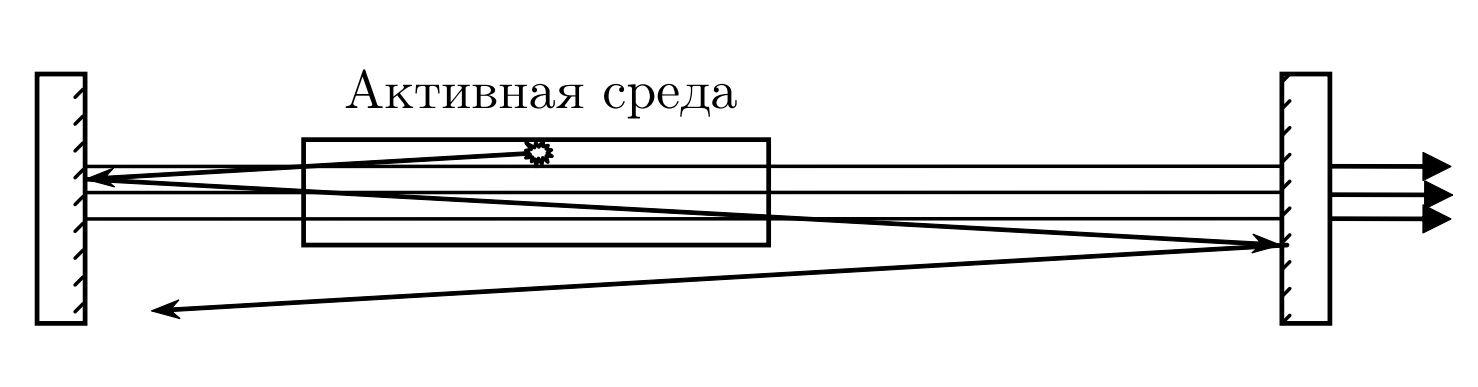
\includegraphics[scale=0.25]{laser1.png}
	\caption{Схема лазера} \label{scheme_laser}
\end{figure}

\paragraph{Условие достижение порога генерации.} Выведем пороговое условие генерации в лазере. 
Для этого рассмотрим простейшую схему лазера, состоящего из плоско-параллельного резонатора (рис. 1),
образованного двумя зеркалами, имеющими коэффициенты отражения $R_1$ и $R_2$, активной среды, 
имеющей усиление $G$ на один проход и дополнительных элементов, размещённых внутри резонатора с 
общим пропусканием $T$ за один проход. Дифракционные потери становятся существенными при малых 
поперечных размерах зеркал или активного элемента, сравнимых с размером одной зоны Френеля для 
расстояния, равного длине резонатора, то есть $r_{las} \approx \sqrt{\lambda L}$. Для получения 
генерации необходимо, чтобы усиление было достаточным для компенсации всех потерь при полном обходе 
резонатора.

\begin{equation}
	R_1R_2T^2G^2 \geq 1 \quad \Rightarrow \quad G \geq \dfrac{1}{T\sqrt{R_1R_2}}
\end{equation}

В непрерывных лазерах в установившемся режиме потери излучения в точности 
компенсируются усилением и усиление активного элемента за один проход равно

\begin{equation}
	G = \dfrac{1}{T\sqrt{R_1R_2}}
\end{equation}

Для того, чтобы лазер имел ненулевую мощность выходного излучения, активный элемент лазера должен
иметь запас по усилению, то есть при отключении положительной обратной связи (удалении зеркал 
резонатора) усиление должно превышать значение, даваемое уравнением (1). При подключении обратной 
связи и выходе на стационарный режим генерации усиление автоматически падает до данной величины.

\paragraph{Гелий-неоновый лазер.} Рассмотрим механизм возникновения усиления в рабочей среде 
гелий-неонового лазера. Лазерная трубка заполняется смесью гелия и неона в соотношении от 5:1 
до 10:1 с общим давлением порядка $10^2$ Па, при котором довольно легко возбудить постоянный 
электрический разряд. Рабочим лазерным веществом является неон. Гелий используется для 
избирательного заселения верхнего рабочего уровня неона. Атомы гелия возбуждаются при столкновениях
с разогнанными в электрическом поле разряда электронами. Передача энергии от возбуждённых атомов 
гелия к атомам неона осуществляется при столкновениях между ними. Известно, что наиболее эффективно
передача энергии от атома к атому происходит в резонансном случае, то есть когда энергии уровней, 
между которыми происходит переход, близки. Упрощённая схема энергетических уровней атомов гелия
и неона изображена на рис. 2.

\begin{figure}[H]
	\centering
	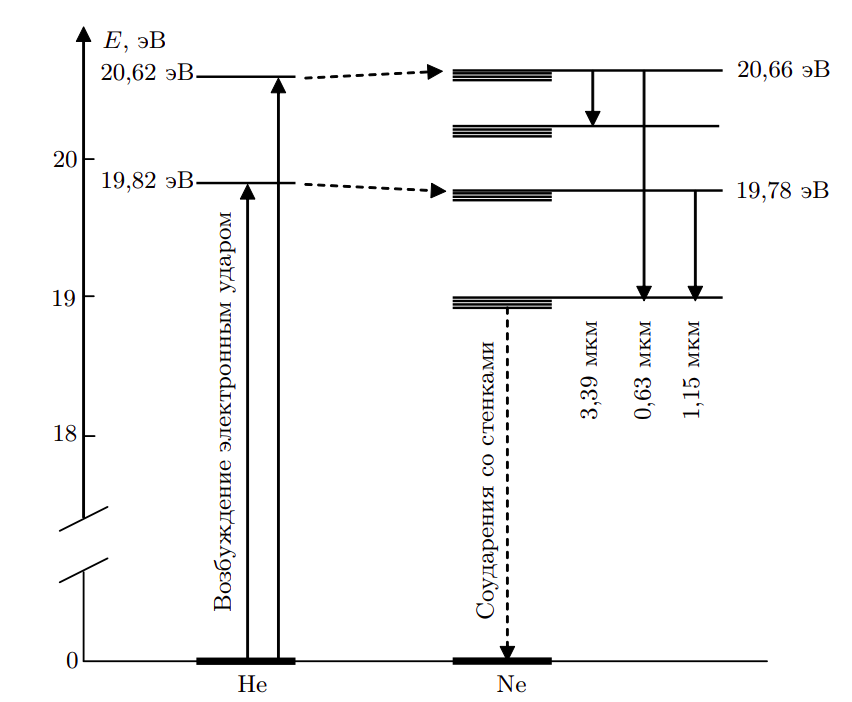
\includegraphics[scale=0.4]{laser2.png}
	\caption{Энергетическая схема работы гелий-неонового лазера} \label{scheme_helium}
\end{figure}

\par На этом рисунке изображена лишь малая часть энергетических уровней неона, в действительности их 
гораздо больше и все они в той или иной степени заселяются в электрическом разряде даже без добавки 
гелия, что может приводить к созданию инверсной населённости между некоторыми уровнями. И 
действительно, генерация лазерного излучения атомами неона получена в лабораторных условиях
на более чем 200 переходах. Однако, во всех промышленных лазерах на неоне для увеличения 
эффективности накачки используют селективное заселение верхних лазерных уровней атомами гелия, 
поэтомуи называются гелий-неоновыми. На рисунке изображены три основных лазерных
перехода с длинами волн 0,63 мкм (красное излучение), а также 1,15 и 3,39 мкм (невидимое 
инфракрасное). 

\par Типичная конструкция гелий-неонового лазера изображена на рис. 3.

\begin{figure}[H]
	\centering
	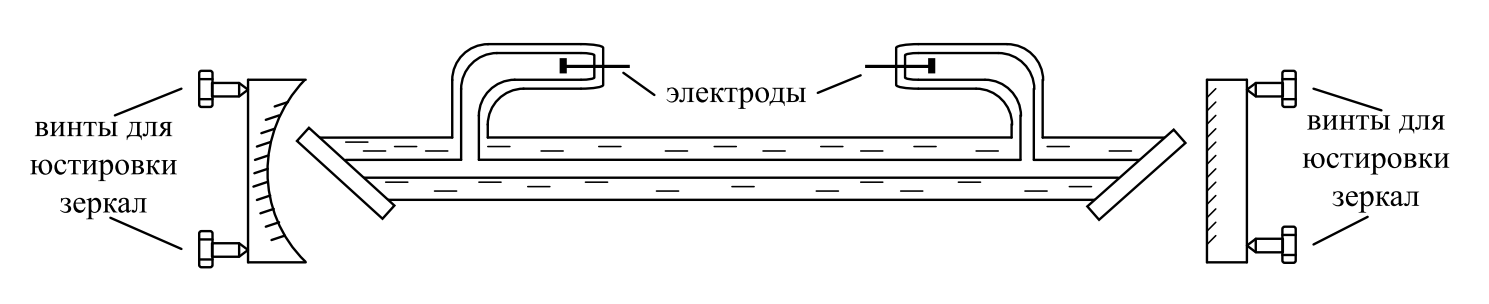
\includegraphics[scale=0.4]{laser3.png}
	\caption{Устройство гелий-неонового лазера} \label{scheme}
\end{figure}

\par Обычно используется сферический или полусферический резонатор, предъявляющий гораздо более мягкие 
требования к точности юстировки зеркал и обеспечивающий повышенную механическую стабильность по
сравнению с плоским резонатором.

\paragraph{Ширина спектра излучения гелий-неонового лазера.} Время жизни верхнего лазерного уровня 
для перехода $0.63$ мкм составляет $10^{-8}$ с.
Из принципа неопределённости $\Delta \nu \cdot \tau \geq 1$ можно получить оценку ширины линии
$\Delta \nu \geq 10^8$ Гц. Реальная ширина спектра генерации обычного гелий-неонового лазера на 
порядок больше. Основной механизм уширения -- эффект Доплера.
В лазерной трубке атомы неона участвуют в хаотическом тепловом движении. Частота излучения 
движущегося источника сдвинута относительно неподвижного источника; в нерелятивистском случае

\begin{equation}
	\Delta \nu = \nu \dfrac{v}{c} \cos \theta
\end{equation}

Поскольку при хаотическом движении $\cos \theta$ принимает значения от 1 до -1, то уширение линии 
приблизительно составляет

\begin{equation}
	\Delta \nu \approx 2\nu \dfrac{v_{ср}}{c} = 2\nu \sqrt{\dfrac{8kT}{\pi m c^2}}
\end{equation}

Точный вывод на основе распределения Максвелла приводит к формуле для полуширины линии

\begin{equation}
	\delta \nu \approx 2\nu \dfrac{v_{ср}}{c} = 2\nu \sqrt{\dfrac{2kT \ln 2}{m c^2}}
\end{equation} 

которая даёт значение на 40\% меньше, чем полученная нами оценочная формула. При температуре 400
K полуширина линии излучения газообразного неона равна $1.5\cdot10^9$ Гц. Полуширина спектра 
лазерного излучения в 2–3 раза меньше этой величины, поскольку вследствие малого коэффициента
усиления генерация происходит только на вершине контура усиления.

\paragraph{Продольные моды.} Рассмотрим более детально спектральный состав излучения гелий-неонового 
лазера. Обычно спектр состоит из нескольких эквидистантных линий, соответствующих различным продольным
модам резонатора. Модами называют стационарные типы колебаний электромагнитного поля в резонаторе.
\par Рассмотрим простейший резонатор из двух зеркал с коэффициентами отражения $R_1$ и
$R_2$ и бесконечно тонкий cлой усиливающего вещества внутри резонатора с усилением
$G$ за один проход. Примем, что состояние лазера стационарно и мощность спонтанного излучения 
слабо зависит от частоты (ширина линии усиления лазерной среды много шире межмодового расстояния, 
что выполняется для гелий-неонового лазера). Чтобы найти мощность излучения внутри резонатора в 
каком-либо месте, например, на внутренней поверхности выходного зеркала, нужно просуммировать после 
последовательных проходов комплексные амплитуды волн, излучаемых лазерной средой в левую сторону 
(получается геометрическая прогрессия), умножить на комплексно-сопряжённую величину, потом проделать
то же для волн, излучаемых в правую сторону и затем сложить. Получается формула

\begin{equation}
	P(\omega) \propto \dfrac{1}{(1 - \sqrt{R}G)^2 + 4\sqrt{R}G\sin^2\frac{\varphi}{2}}
\end{equation} 

где $R = R_1R_2$, $\varphi$ -- набег фазы при полном обходе резонатора. Эта функция имеет резкие 
максимумы при $\varphi = 2\pi n$, поскольку в стационарном состоянии $\sqrt{R}G \approx 1$.
Таким образом, для многослойных диэлектрических зеркал, также как и для металлических, набег 
фазы при полном обходе резонатора должен быть кратен $2\pi$.

\begin{figure}[H]
	\begin{minipage}[h]{0.49\linewidth}
		\center{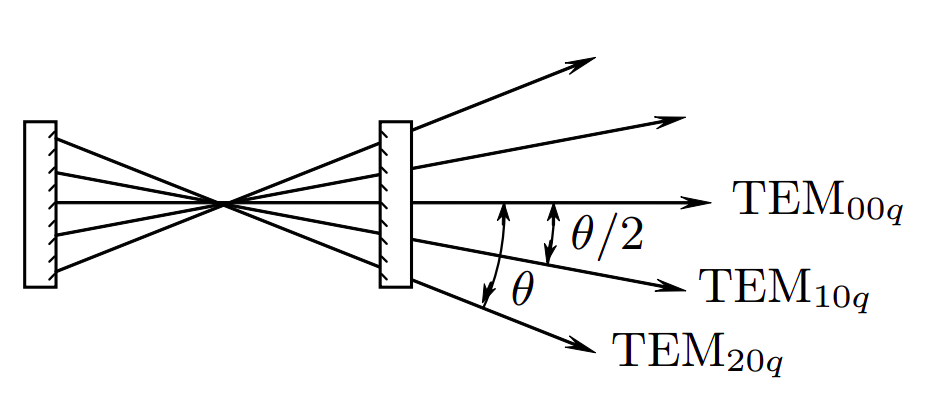
\includegraphics[width=0.95\linewidth]{laser4.png}}
		\caption{Направления распространения мод с разными поперечными индексами (согласно простейшей теории Шавлова и Таунса)}
	\end{minipage}
	\begin{minipage}[h]{0.49\linewidth}
		\center{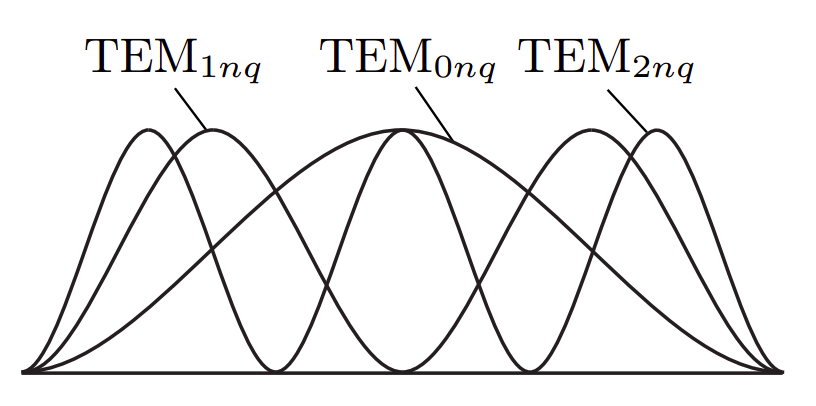
\includegraphics[width=0.95\linewidth]{laser5.png}}
		\caption{Распределение интенсивности лазерного излучения на
		зеркале резонатора по одной из
		поперечных координат для трёх
		низших поперечных мо
		д (согласно простейшей теории Шавлова
		и Таунса)}
	\end{minipage}
\end{figure}

\paragraph{Поперечные моды.} Для обращения интенсивности в ноль на краях зеркала необходимо, 
чтобы на ширине зеркала $D$ укладывалось целое число периодов, поэтому $\theta = \pm m \frac{\lambda}{2} D$.
Такое же условие должно выполняться по второй координате в плоскости зеркала:
$\theta = \pm p \frac{\lambda}{2} D$. Здесь $m$ и $p$ -- целые числа. Результирующий угол равен:

\begin{equation}
	\theta = \pm \sqrt{m^2 + p^2} \dfrac{\lambda}{2} D \approx \pm \sqrt{m^2 + p^2} \; \dfrac{\theta_{\text{дифр}}}{2}
\end{equation} 

где $\theta_{\text{дифр}} \approx \lambda / D$ -- дифракционная расходимость лазерного 
пучка с поперечным размером $D$.

\par На рис. 4 и 5 схематически показаны направления распространения разных поперечных мод
и распределение интенсивности излучения на зеркале по одной из поперечных координат.
Найдём сдвиг частоты поперечных мод относительно чисто продольных. Для моды $ТЕМ_{mpq}$, 
распространяющейся под углом $\theta$ к оси резонатора составляющая волнового вектора по 
оси резонатора равна $k_z = q\pi L$, где $L$ -- длина резонатора. Составляющая в плоскости 
зеркал равна $k_{x,y} = k \sin \theta \approx k_z \theta$. Учитывая, что $m,p \ll q$, 
$\theta \ll 1$, $\omega = kc$ и используя выражение (3), для $\theta$ нетрудно получить:

\begin{equation}
	\omega_{mpq} \approx \omega_{00q}\left[1 + \dfrac{1}{8}(m^2 + p^2)\dfrac{\lambda^2}{D^2}\right]
\end{equation} 

Полезно оценить разницу частот чисто продольной моды и поперечной моды с такимже продольным 
индексом и сравнить её с межмодовым расстоянием для продольных мод. Учитывая, что 
$\omega_{00q} \approx 2\pi c/\lambda$, где $lambda$ -- средняя длина волны лазерного излучения, 
получим:

\begin{equation}
	\dfrac{\omega_{mpq} - \omega_{00q}}{\omega_{00q+1} - \omega_{00q}} \approx (m^2 + p^2)\dfrac{\lambda L/4}{D^2}
\end{equation} 

В случае типичного гелий-неонового лазера для низшей поперечной моды ($m = 1$, $p = 0$) имеем:
\begin{equation}
	\dfrac{\omega_{10q} - \omega_{00q}}{\omega_{00q+1} - \omega_{00q}} \approx 10^{-2}
\end{equation} 

Это означает, что спектр мод с ненулевыми поперечными индексами лишь незначительно сдвинут относительно 
спектра чисто продольных мод, этот сдвиг составляет единицы процентов от межмодового расстояния и 
не разрешается большинством спектральных приборов.

\begin{figure}[H]
	\begin{minipage}[h]{0.3\linewidth}
		\center{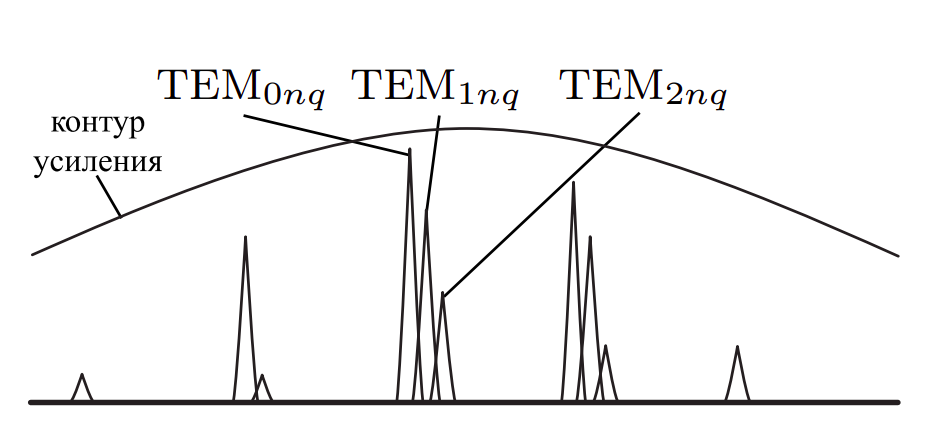
\includegraphics[width=0.95\linewidth]{laser6.png}}
		\caption{Примерный вид спектра излучения гелий неонового лазер}
	\end{minipage}
	\begin{minipage}[h]{0.7\linewidth}
		\center{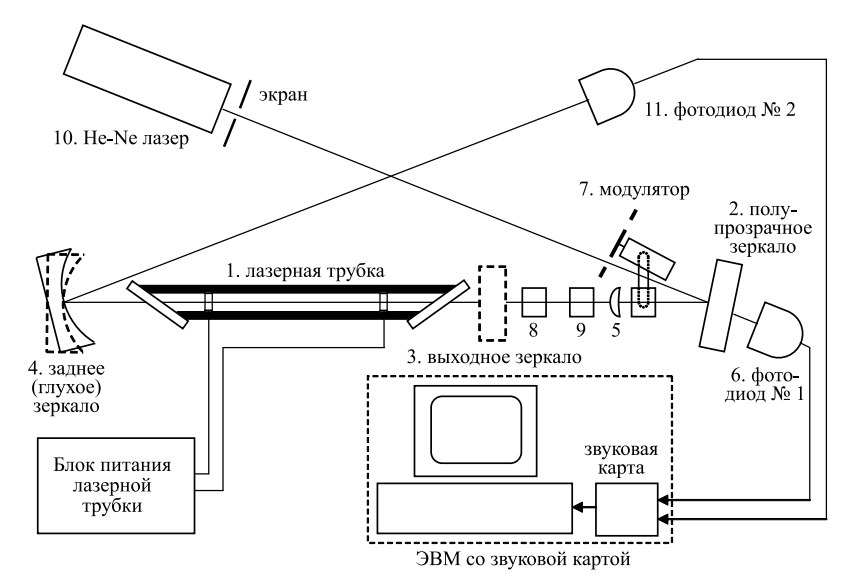
\includegraphics[width=0.95\linewidth]{laser7.png}}
		\caption{Схема установки. Штриховыми линиями показано положение
		зеркал при получении лазерной генерации на исследуемой трубке}
	\end{minipage}
\end{figure}

\paragraph{Экспериментальная установка.} Схема экспериментальной установки приведена на рис. 7. 
На оптической скамье расположены: газоразрядная трубка исследуемого He-Ne лазера ЛГ-75 (1), 
рейтера для крепления юстировочных оправ с зеркалами (2, 3, 4), линза, уменьшающая расходимость 
юстировочного лазера (5), фотодиод (6), модулятор (7) а также съемный рейтер (8) с отрицательной 
линзой для наблюдения модовой структуры излучения исследуемого лазера и рейтер (9), в который 
вставляется либо экран, либо поляроид. Юстировочный лазер (10) и фотодиод (11) закреплены на 
столе. Модулятор может быть повёрнут в разные положения: при измерении коэффициента усиления он 
модулирует пучок, идущий от юстировочного лазера, при измерении поляризации излучения 
исследуемого лазера он модулирует это излучение а в остальных случаях он отводится в сторону, 
чтобы не перекрывать пучки. Юстировочный лазер предназначен для юстировки всех элементов установки
и для измерения коэффициента усиления активной среды исследуемого лазера. 
\par Поскольку коэффициент усиления на рабочей частоте лазера мал, и усиление интенсивности луча 
зондирующего лазера при длине трубки $\approx 1$м составляет всего несколько процентов,
в данной работе измеряется одновременно интенсивность излучения до и после
прохождения исследуемой среды. Этот метод позволяет исключить влияние
нестабильности интенсивности зондирующего лазера во времени, которое составляет
обычно несколько процентов. Сигналы с обоих фотодиодов подаются на звуковую
карту компьютера, и с помощью программы PhysLab измеряются с высокой точностью.
Для настройки резонатора исследуемого лазера используются зеркала, закреплённые
в съемных юстируемых оправах. Изучение поляризации исследуемого лазера, его
модовой структуры производится с помощью поляроида и короткофокусной линзы.
Перед проведением измерений ознакомитесь с приложением, в котором описано
использование программы PhysLab для измерений интенсивности света и методика
измерения коэффициента усиления лазерной трубки.

\section{Ход работы}

\subsection{Поляризация исследуемого лазера}
\par Исследуем поляризацию исследуемого лазера, измерив зависимость интенсивности излучения от угла поворота поляроида.
Оценим погрешности:
$$\Delta \theta=2^{\circ} \qquad \qquad \delta I = 50~\text{мкВ}$$

\begin{figure}[H]
	\centering
	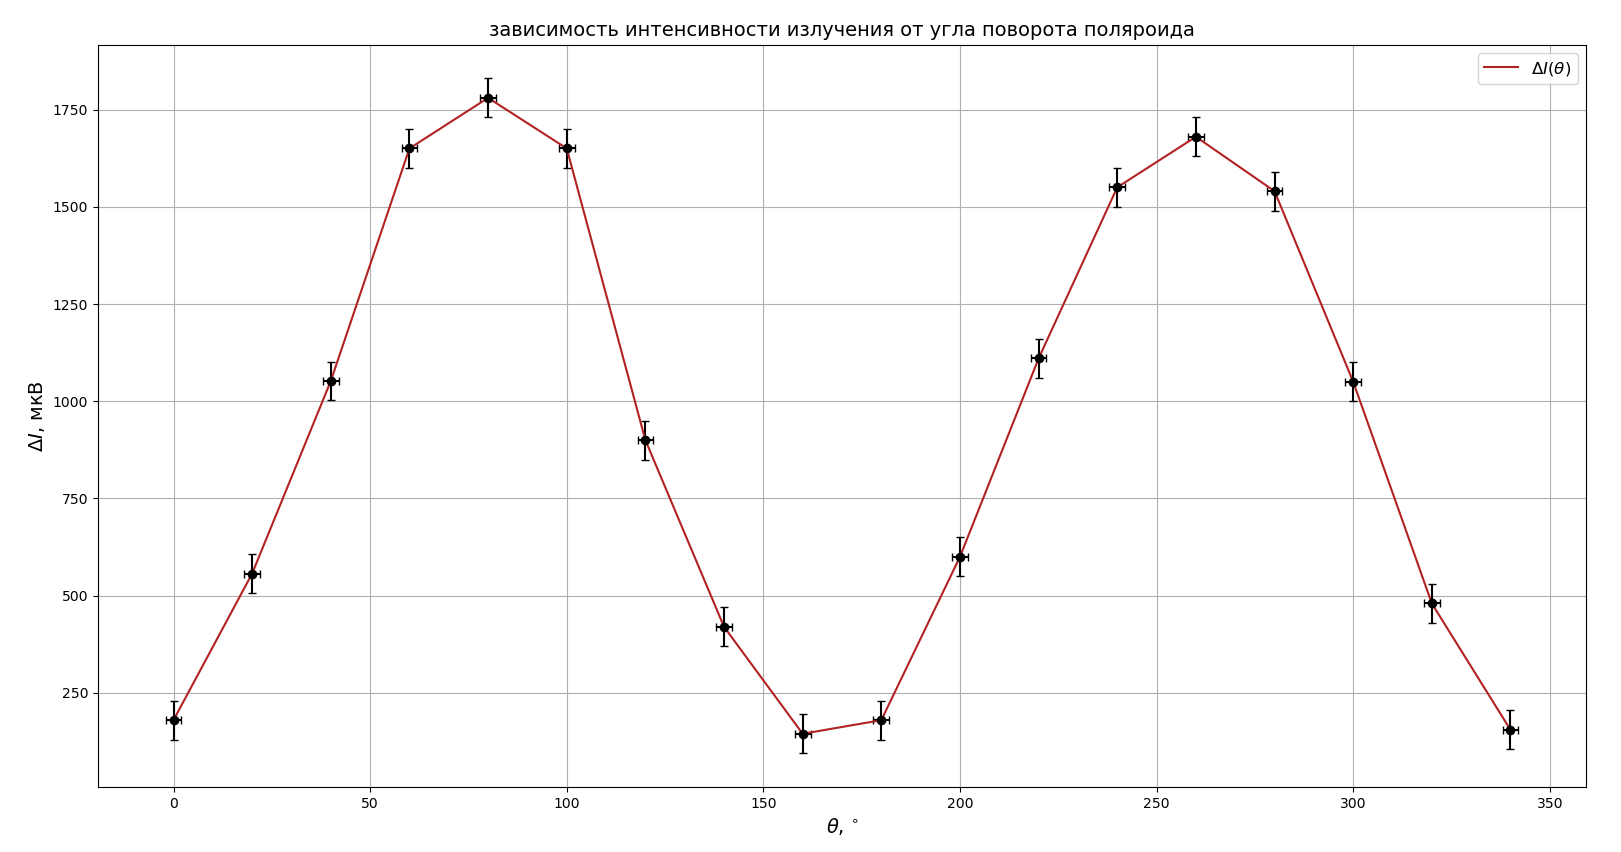
\includegraphics[scale=0.4]{graph.png}
\end{figure}

\begin{table}[h]
	\centering
	\caption{зависимость интенсивности излучения от угла поворота поляроида.}
	\begin{tabular}{|*{4}{l|}} \hline
		$\theta$, $^{\circ}$ & $I_1$, мкВ & $I_2$, мкВ & $\Delta I$, мкВ  \\ \hline
		$0$   & $480$  &  $300$ & $180$  \\ \hline
		$20$  & $744$  &  $187$ & $557$  \\ \hline
		$40$  & $1100$ &   $48$ & $1052$  \\ \hline
		$60$  & $1500$ & $-150$ & $1650$  \\ \hline
		$80$  & $1600$ & $-180$ & $1780$  \\ \hline
		$100$ & $1500$ & $-150$ & $1650$  \\ \hline
		$120$ & $1000$ &  $100$ & $900$  \\ \hline
		$140$ & $670$  &  $250$ & $420$  \\ \hline
		$160$ & $450$  &  $305$ & $145$  \\ \hline
		$180$ & $480$  &  $300$ & $180$  \\ \hline
		$200$ & $750$  &  $150$ & $600$  \\ \hline
		$220$ & $1100$ &  $-10$ & $1110$  \\ \hline
		$240$ & $1400$ & $-150$ & $1550$  \\ \hline
		$260$ & $1500$ & $-180$ & $1680$  \\ \hline
		$280$ & $1400$ & $-140$ & $1540$  \\ \hline
		$300$ & $1100$ &   $50$ & $1050$  \\ \hline
		$320$ & $750$  &  $270$ & $480$  \\ \hline
		$340$ & $500$  &  $345$ & $155$  \\ \hline
	\end{tabular}
\end{table}

\subsection{Наблюдение модовой структуры лазерного излучения}

\begin{figure}[H]
	\begin{minipage}[h]{0.5\linewidth}
		\center{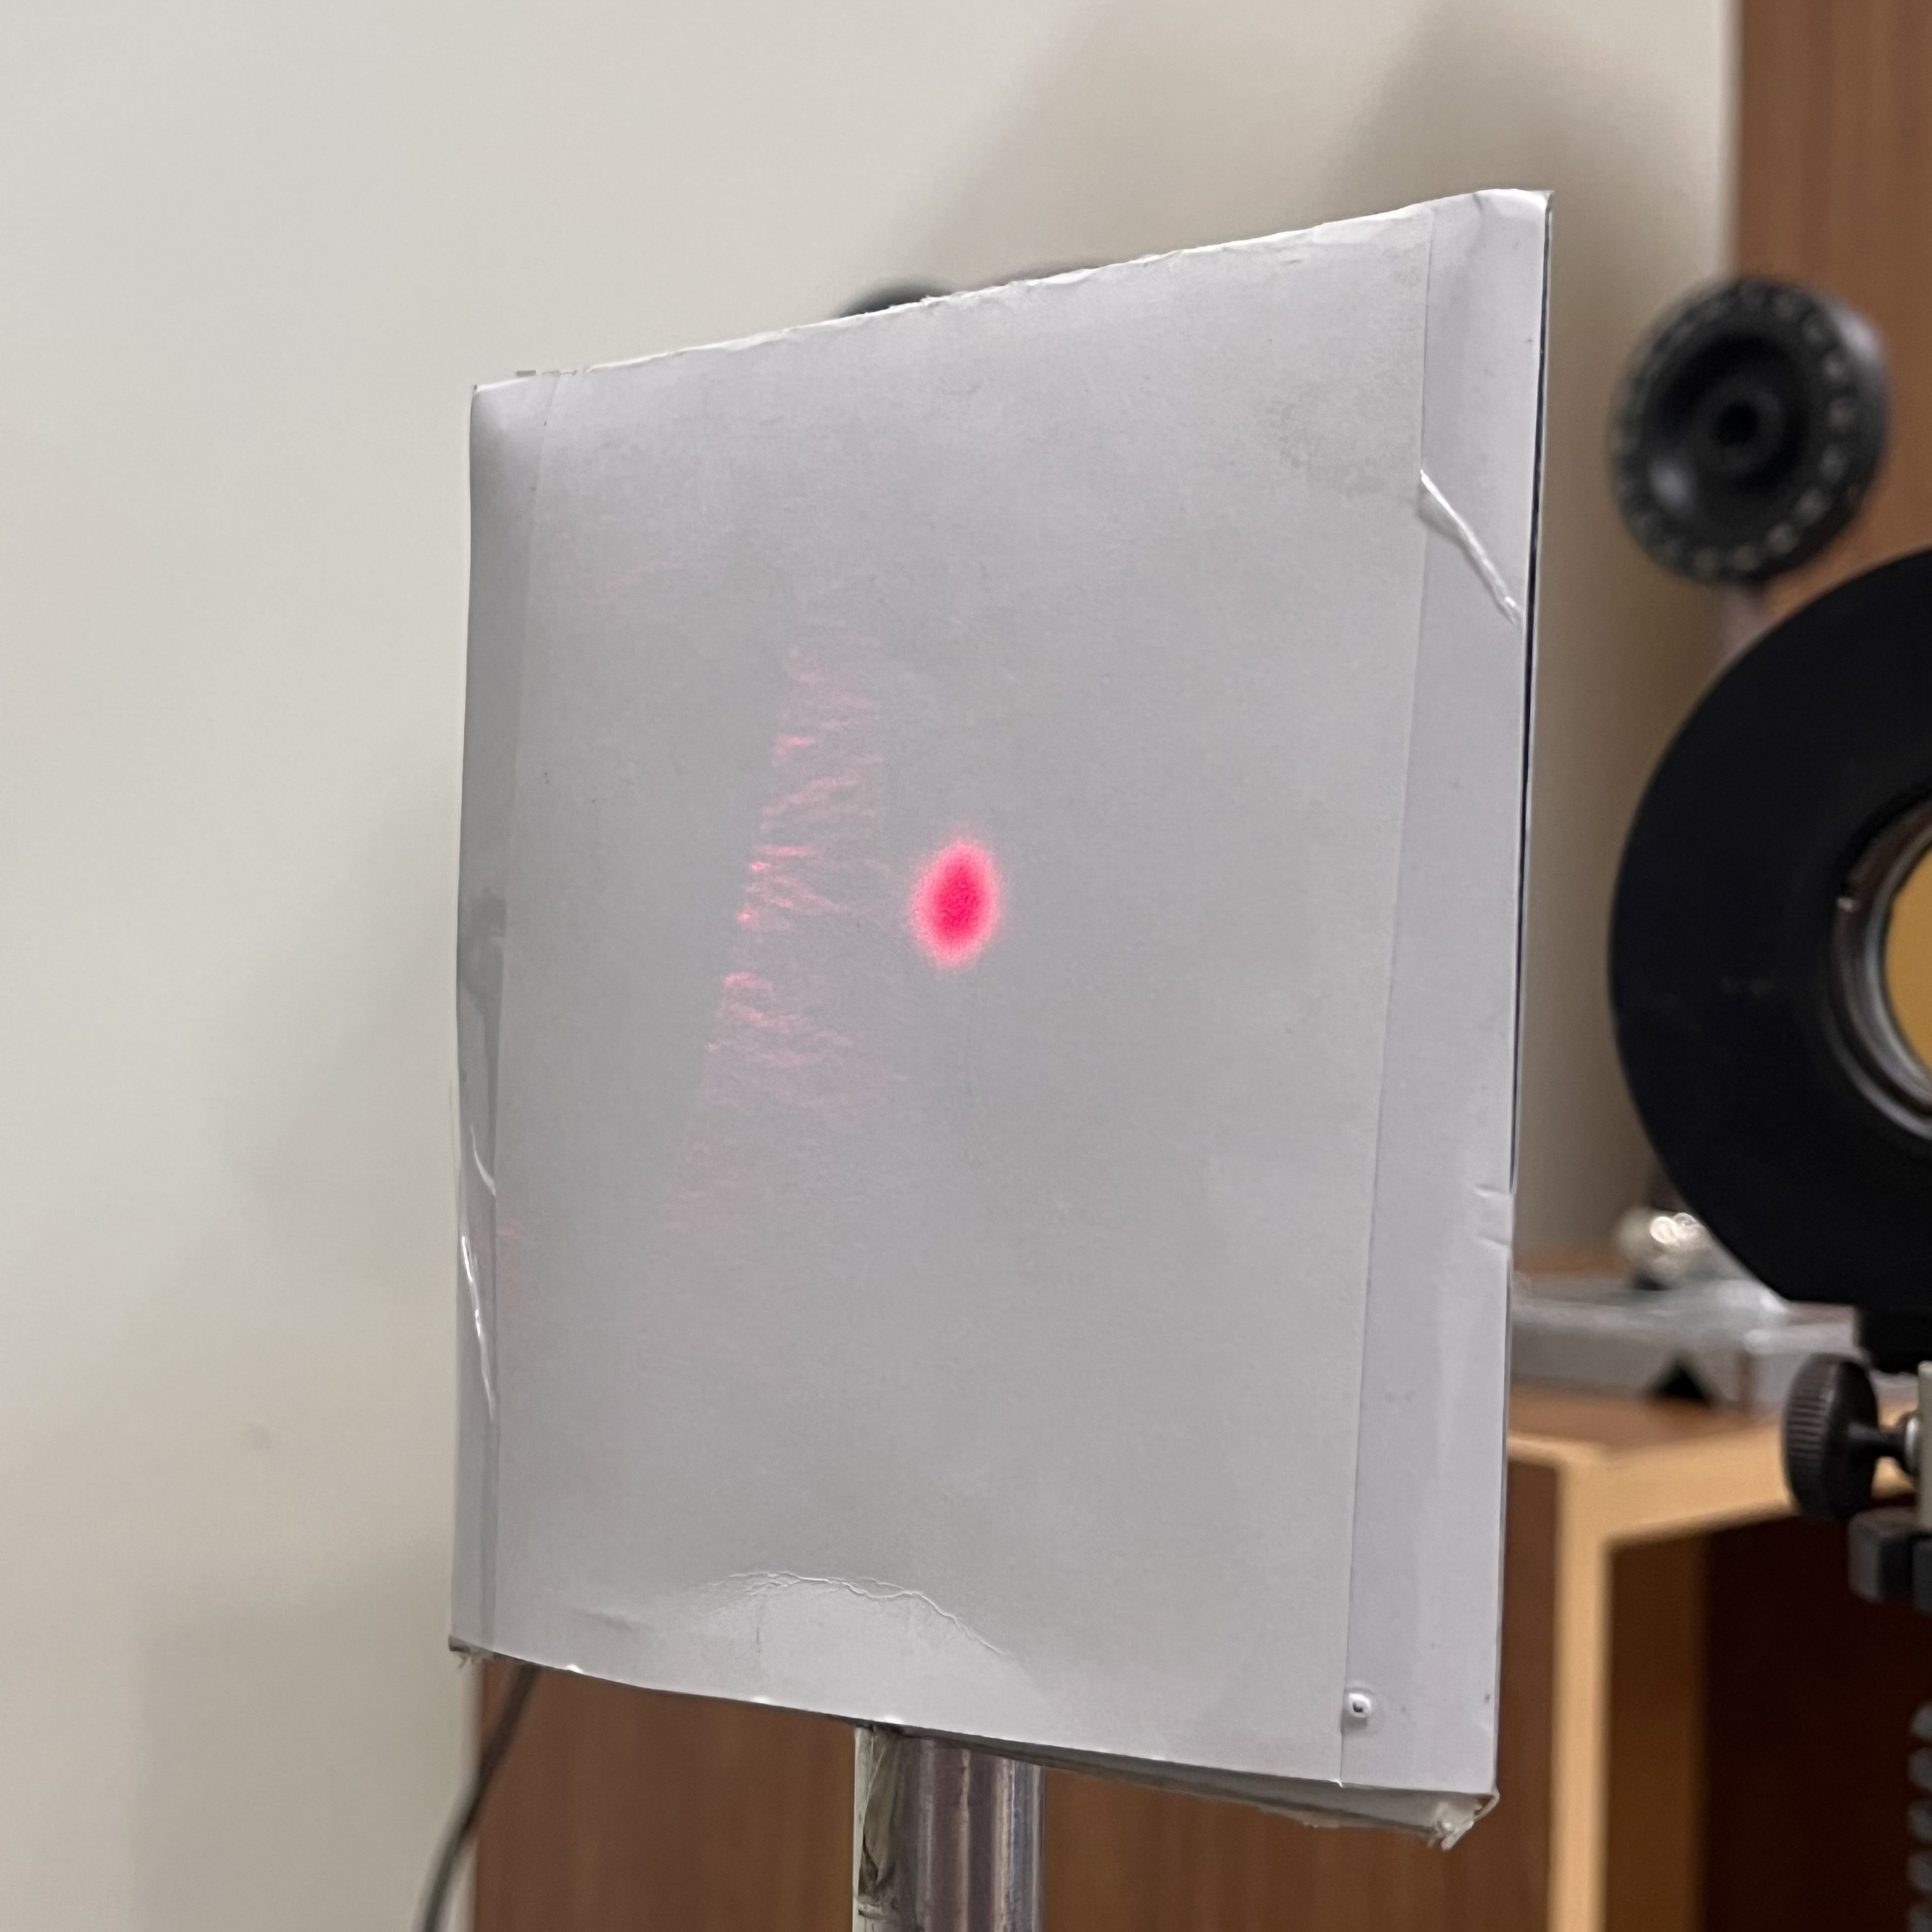
\includegraphics[width=1\linewidth]{1.JPG}}
		\caption{Одномодовый режим}
	\end{minipage}
	\begin{minipage}[h]{0.5\linewidth}
		\center{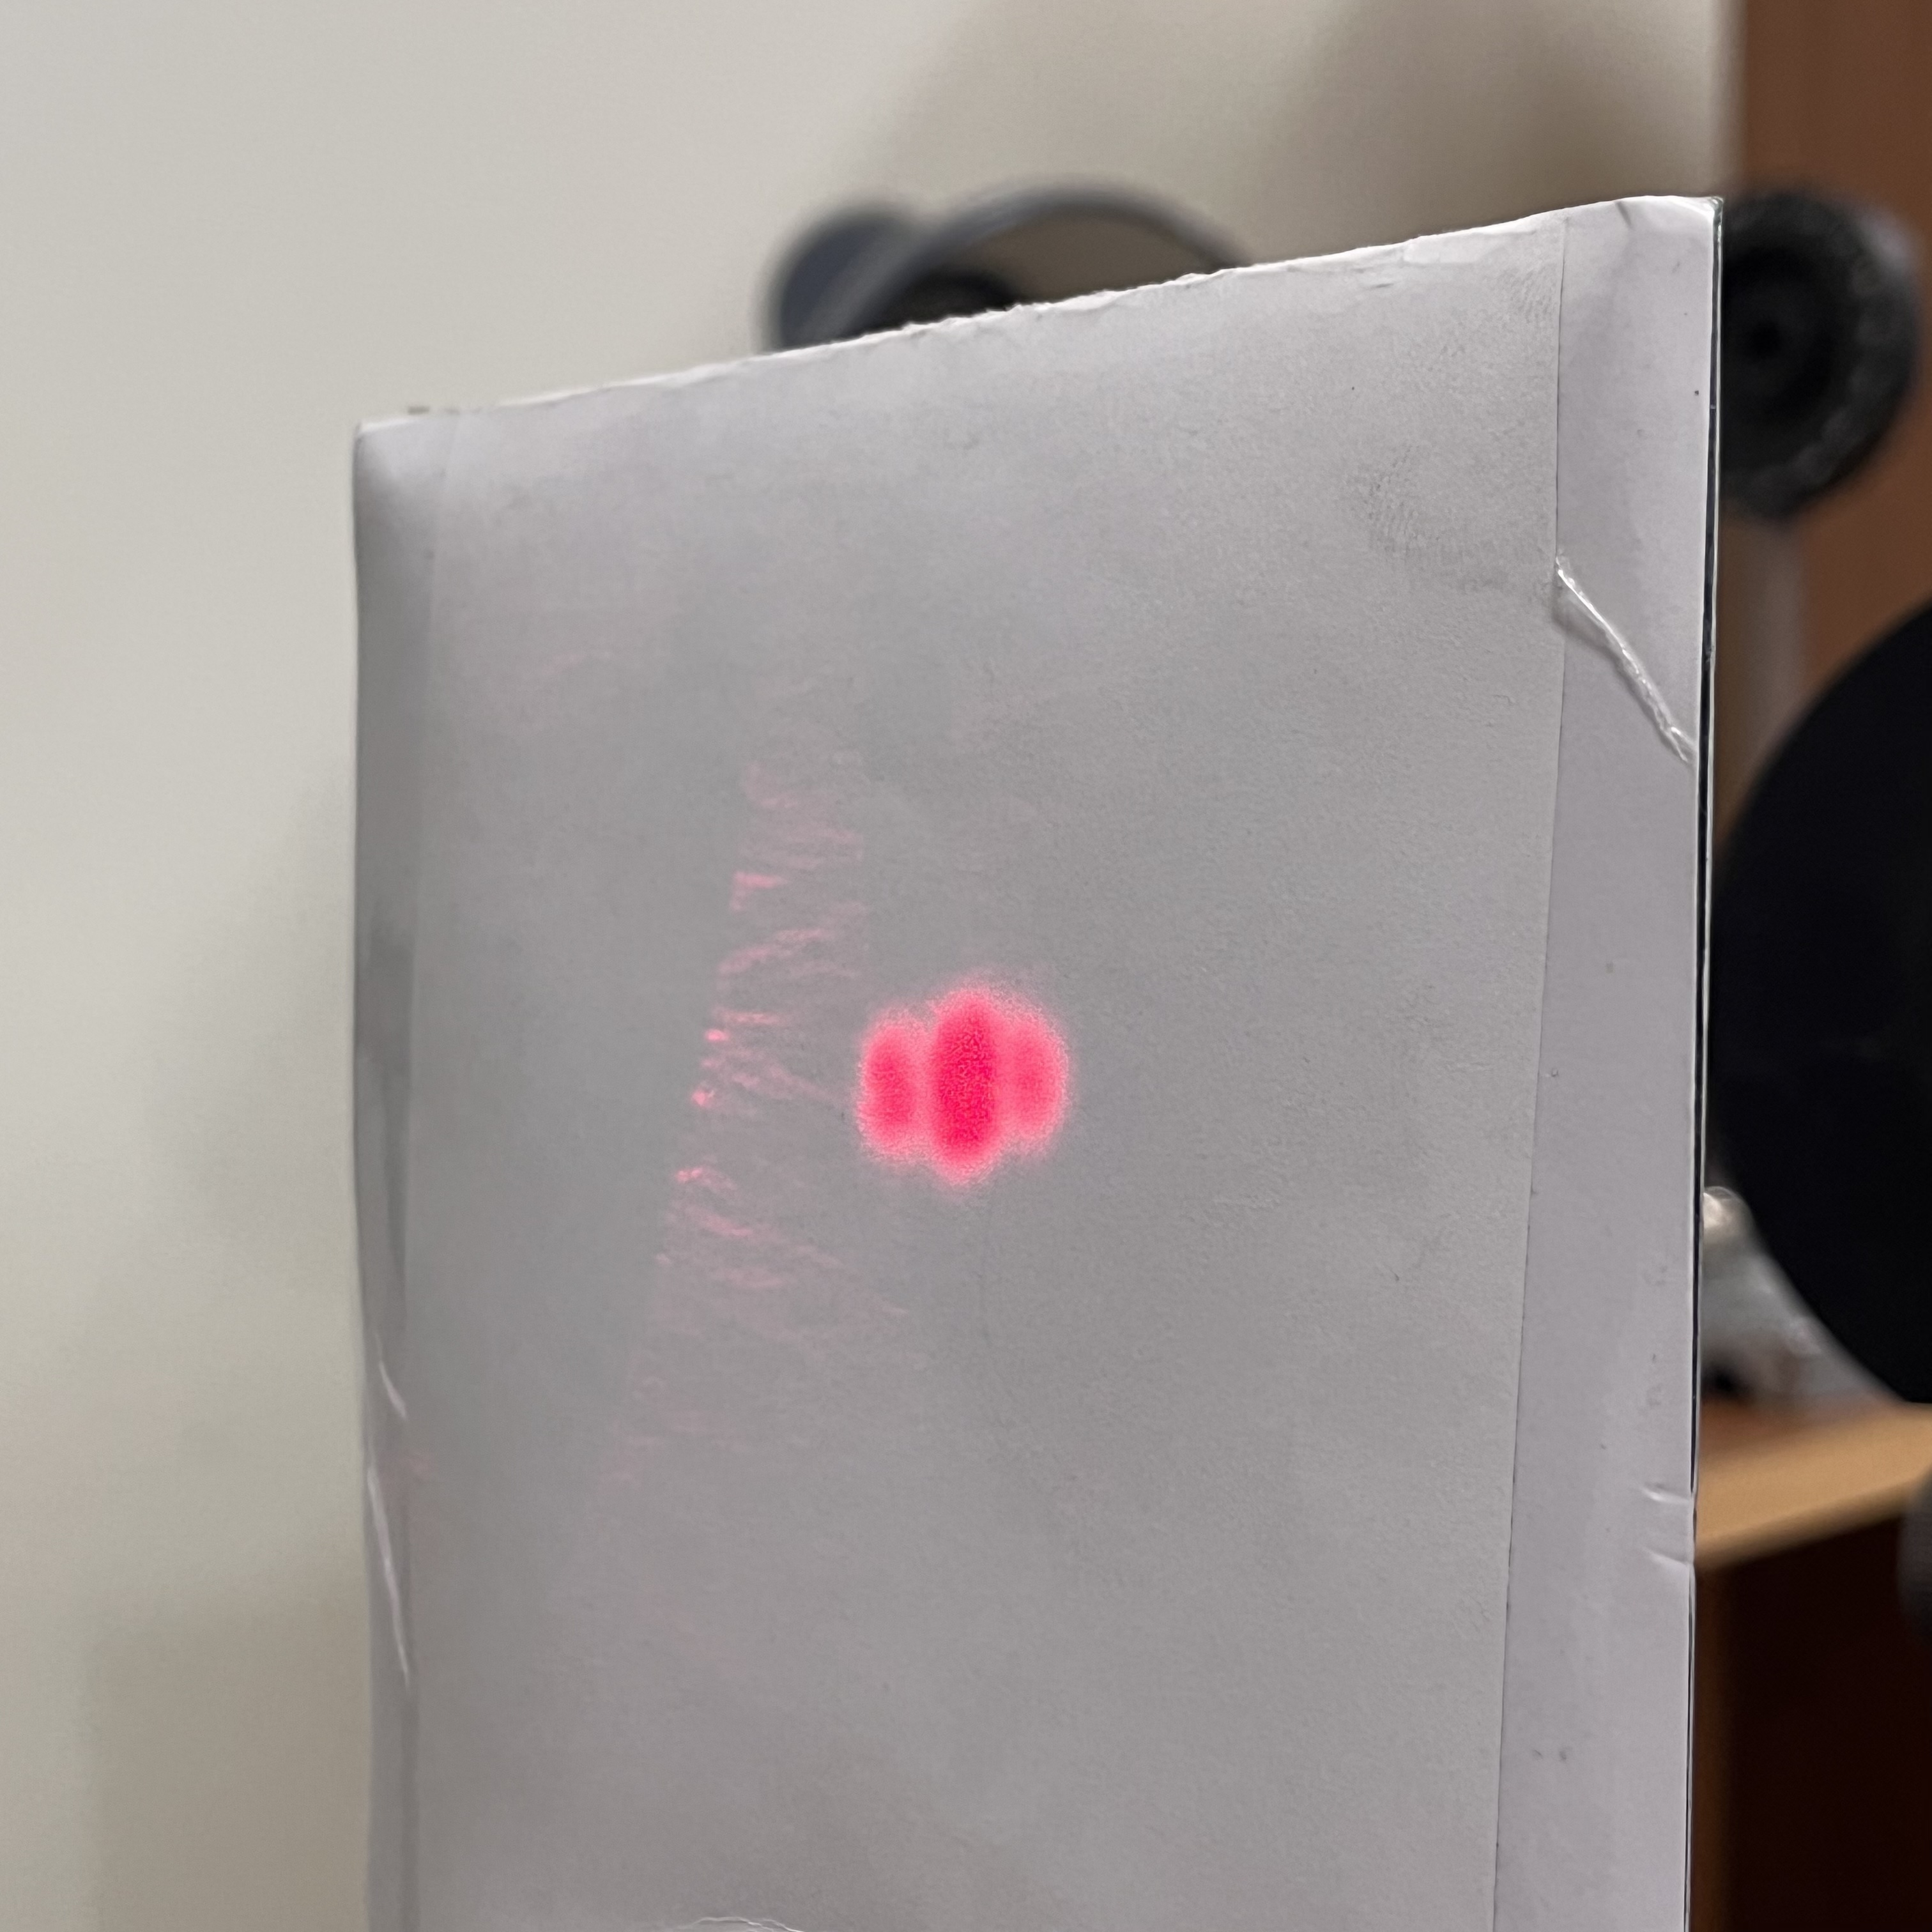
\includegraphics[width=1\linewidth]{2.JPG}}
		\caption{Трёхмодовый режим}
	\end{minipage}
\end{figure}

\begin{figure}[H]
	\begin{minipage}[h]{0.5\linewidth}
		\center{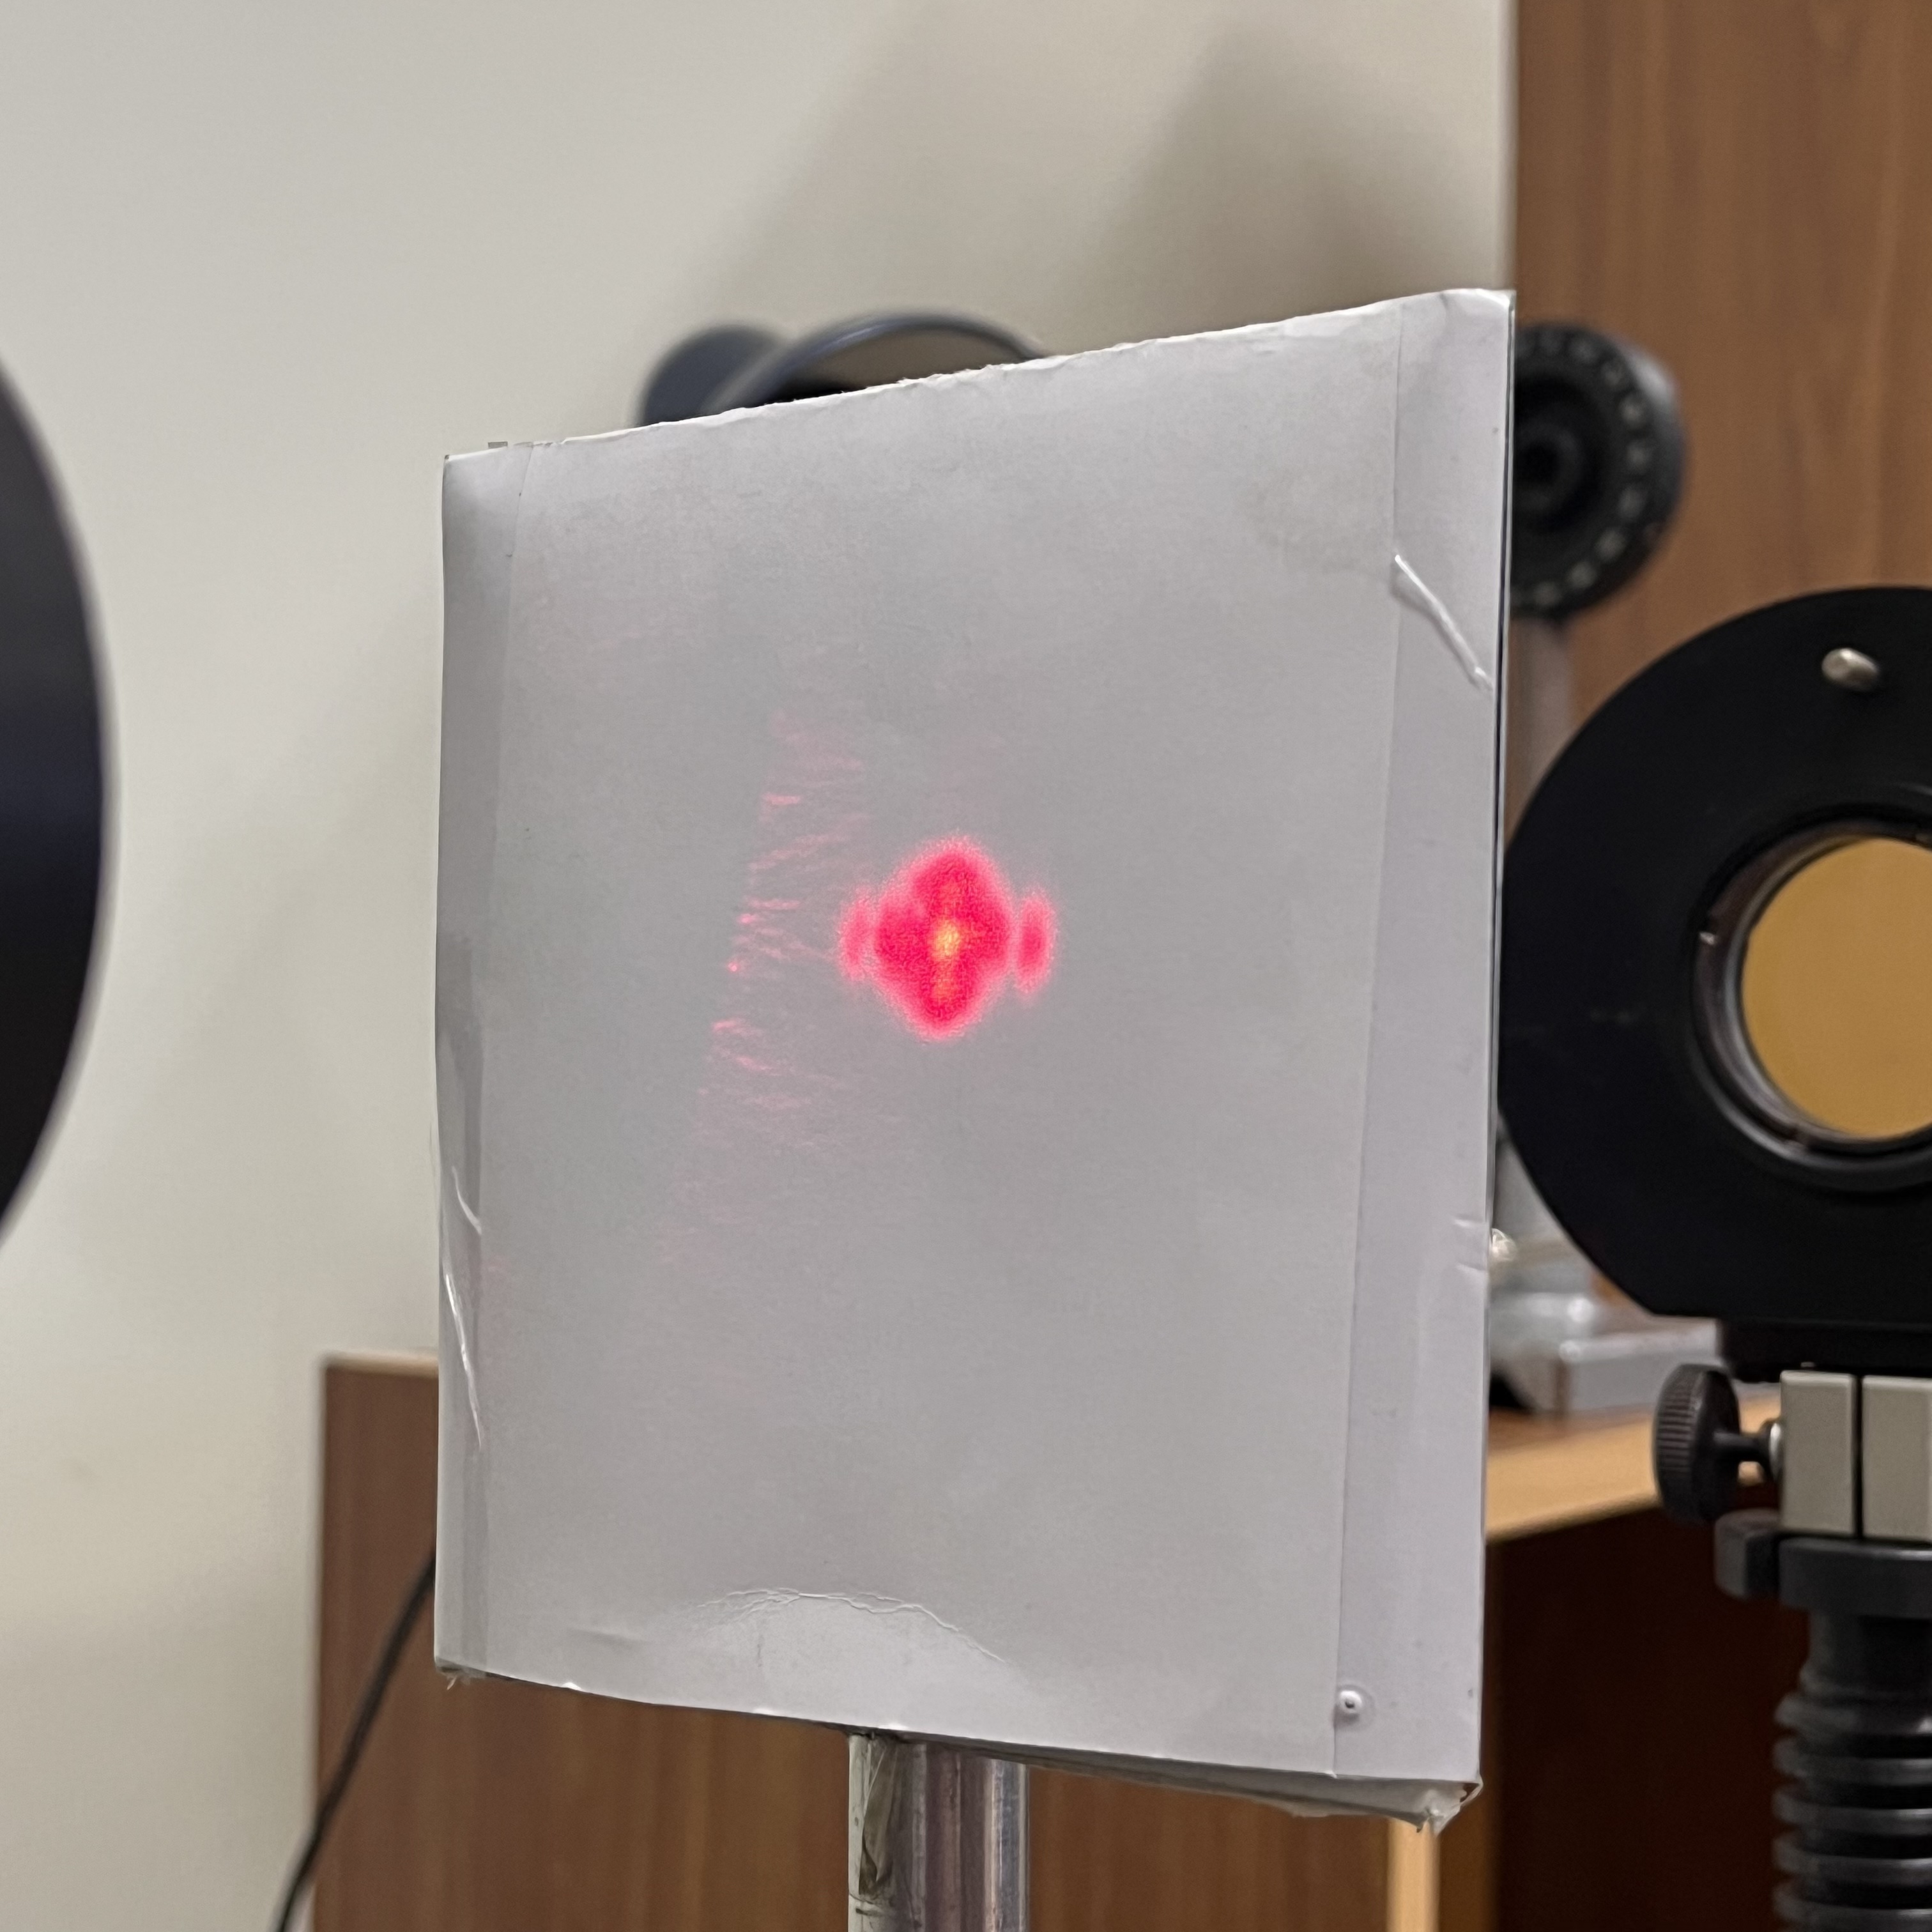
\includegraphics[width=1\linewidth]{3.JPG}}
		\caption{Многомодовый режим 1}
	\end{minipage}
	\begin{minipage}[h]{0.5\linewidth}
		\center{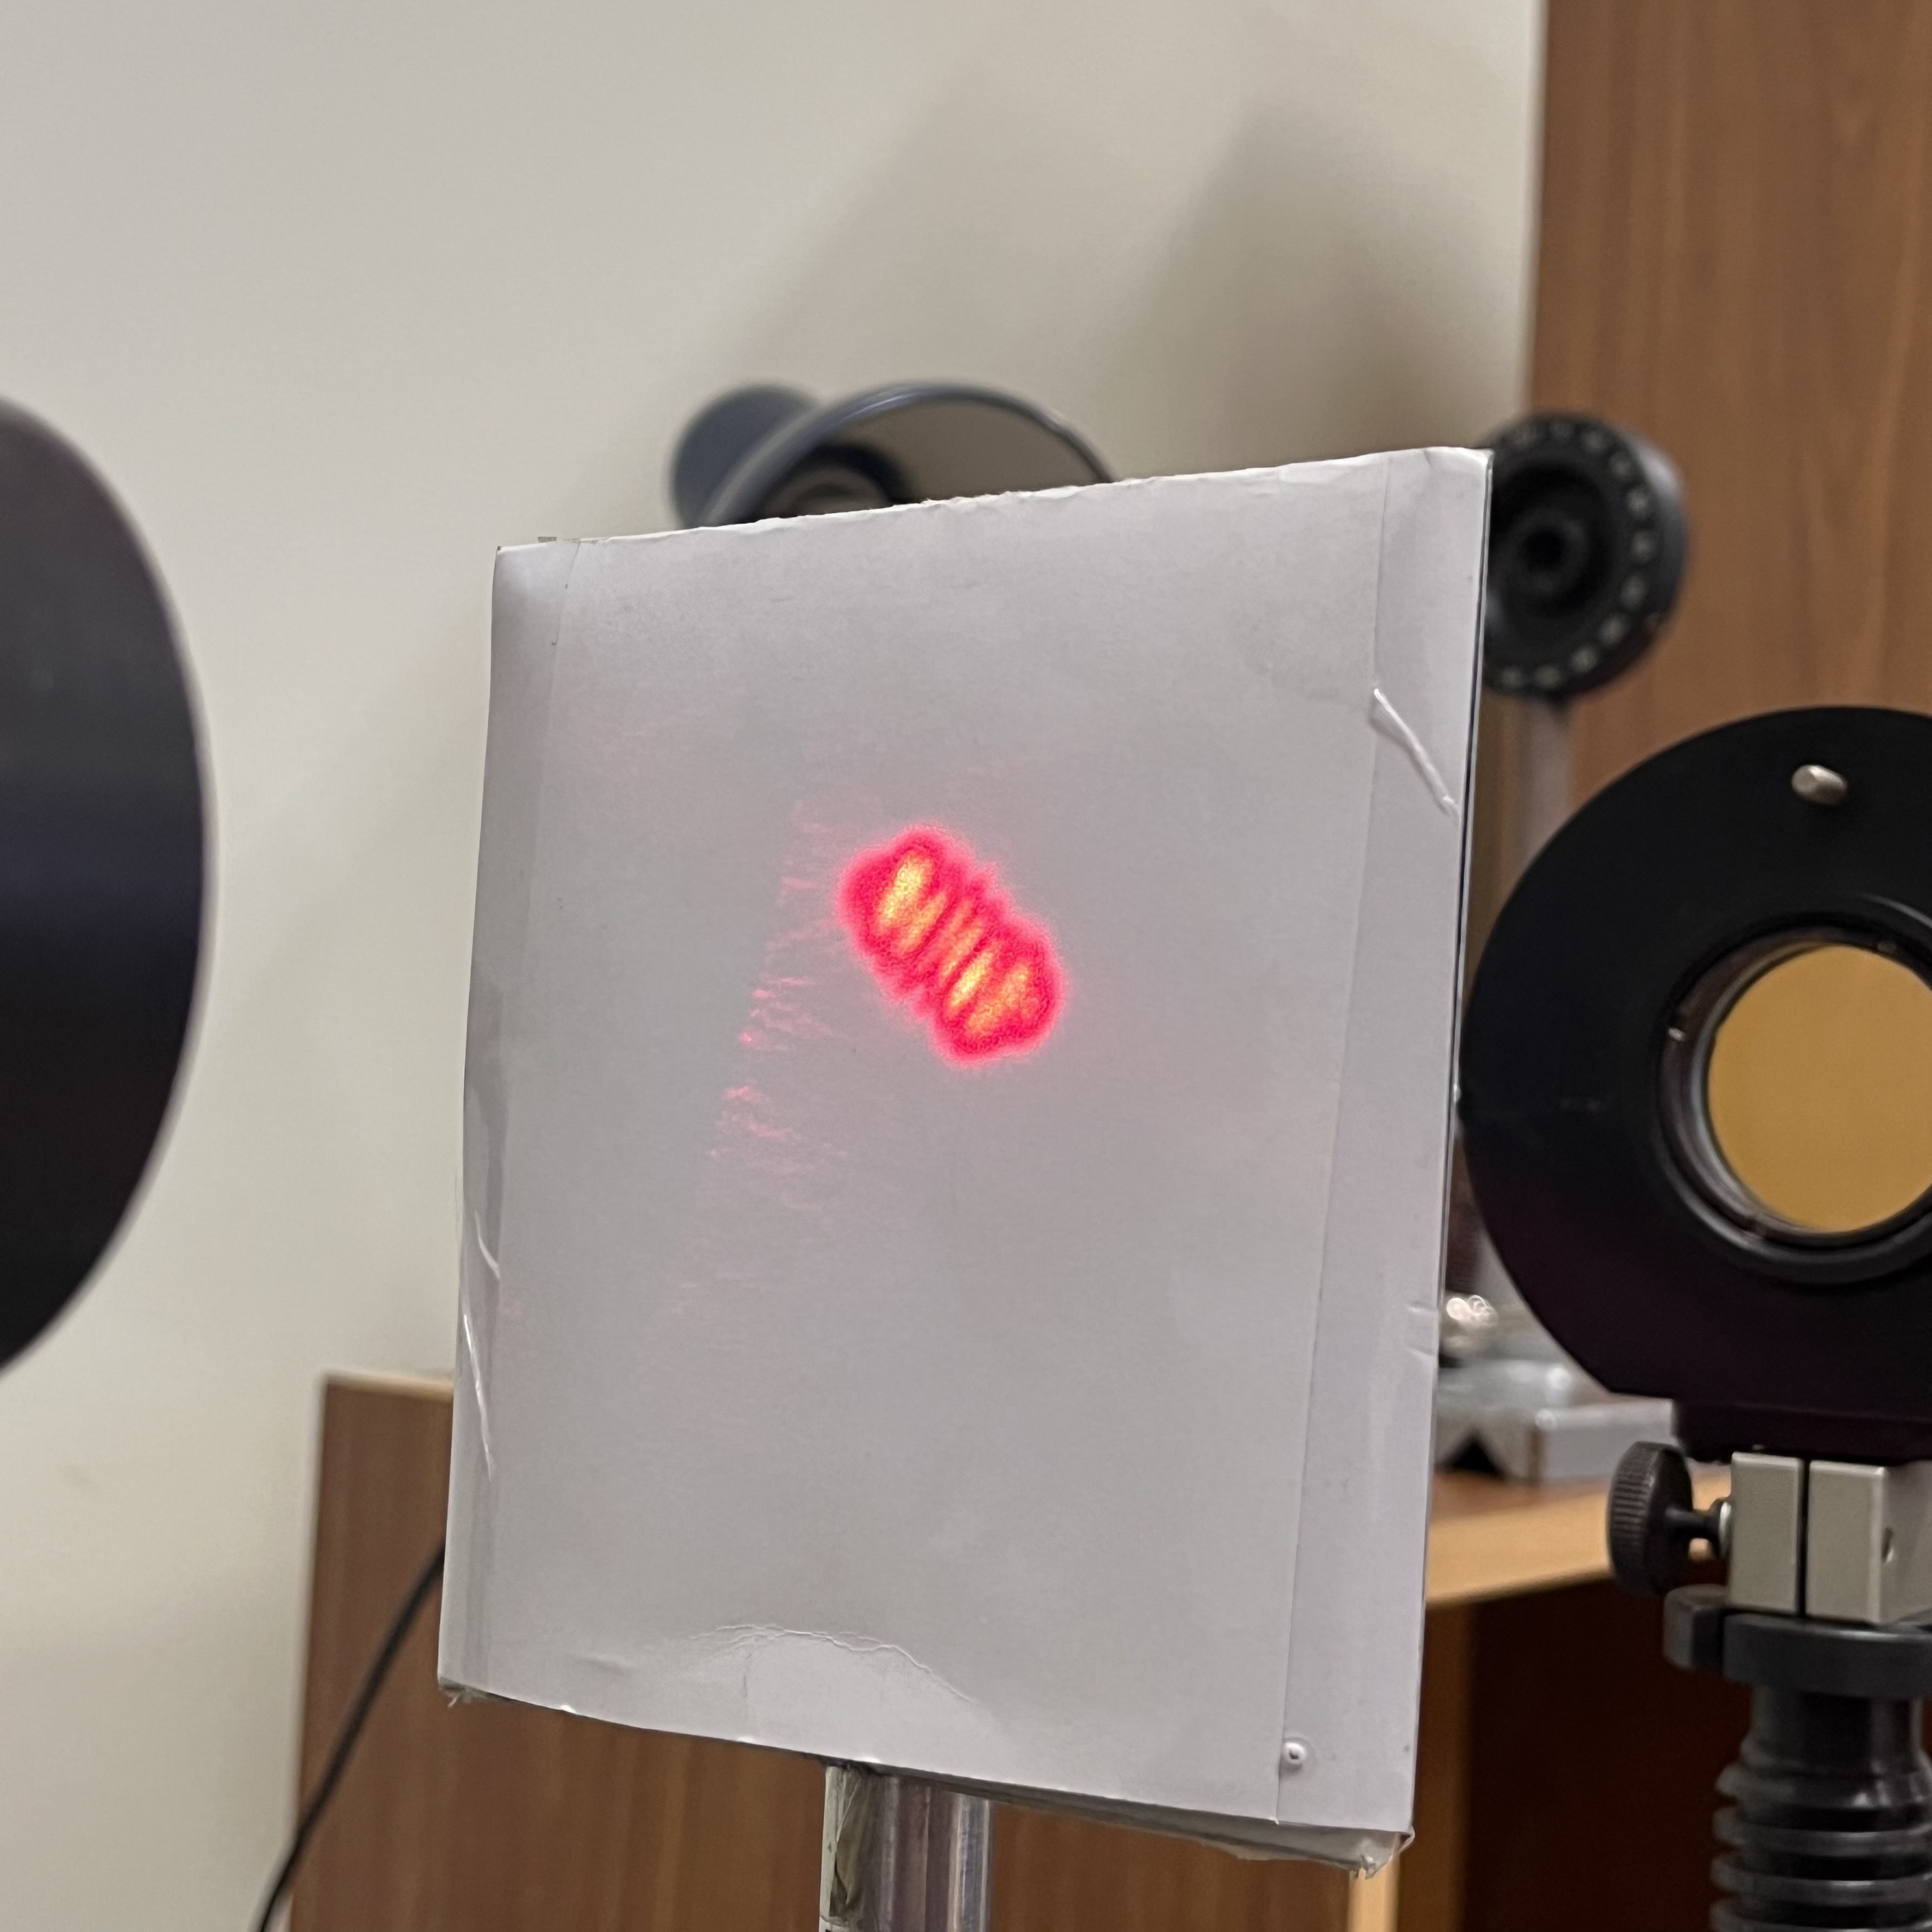
\includegraphics[width=1\linewidth]{4.JPG}}
		\caption{Многомодовый режим 2}
	\end{minipage}
\end{figure}

\begin{figure}[H]
	\begin{minipage}[h]{0.5\linewidth}
		\center{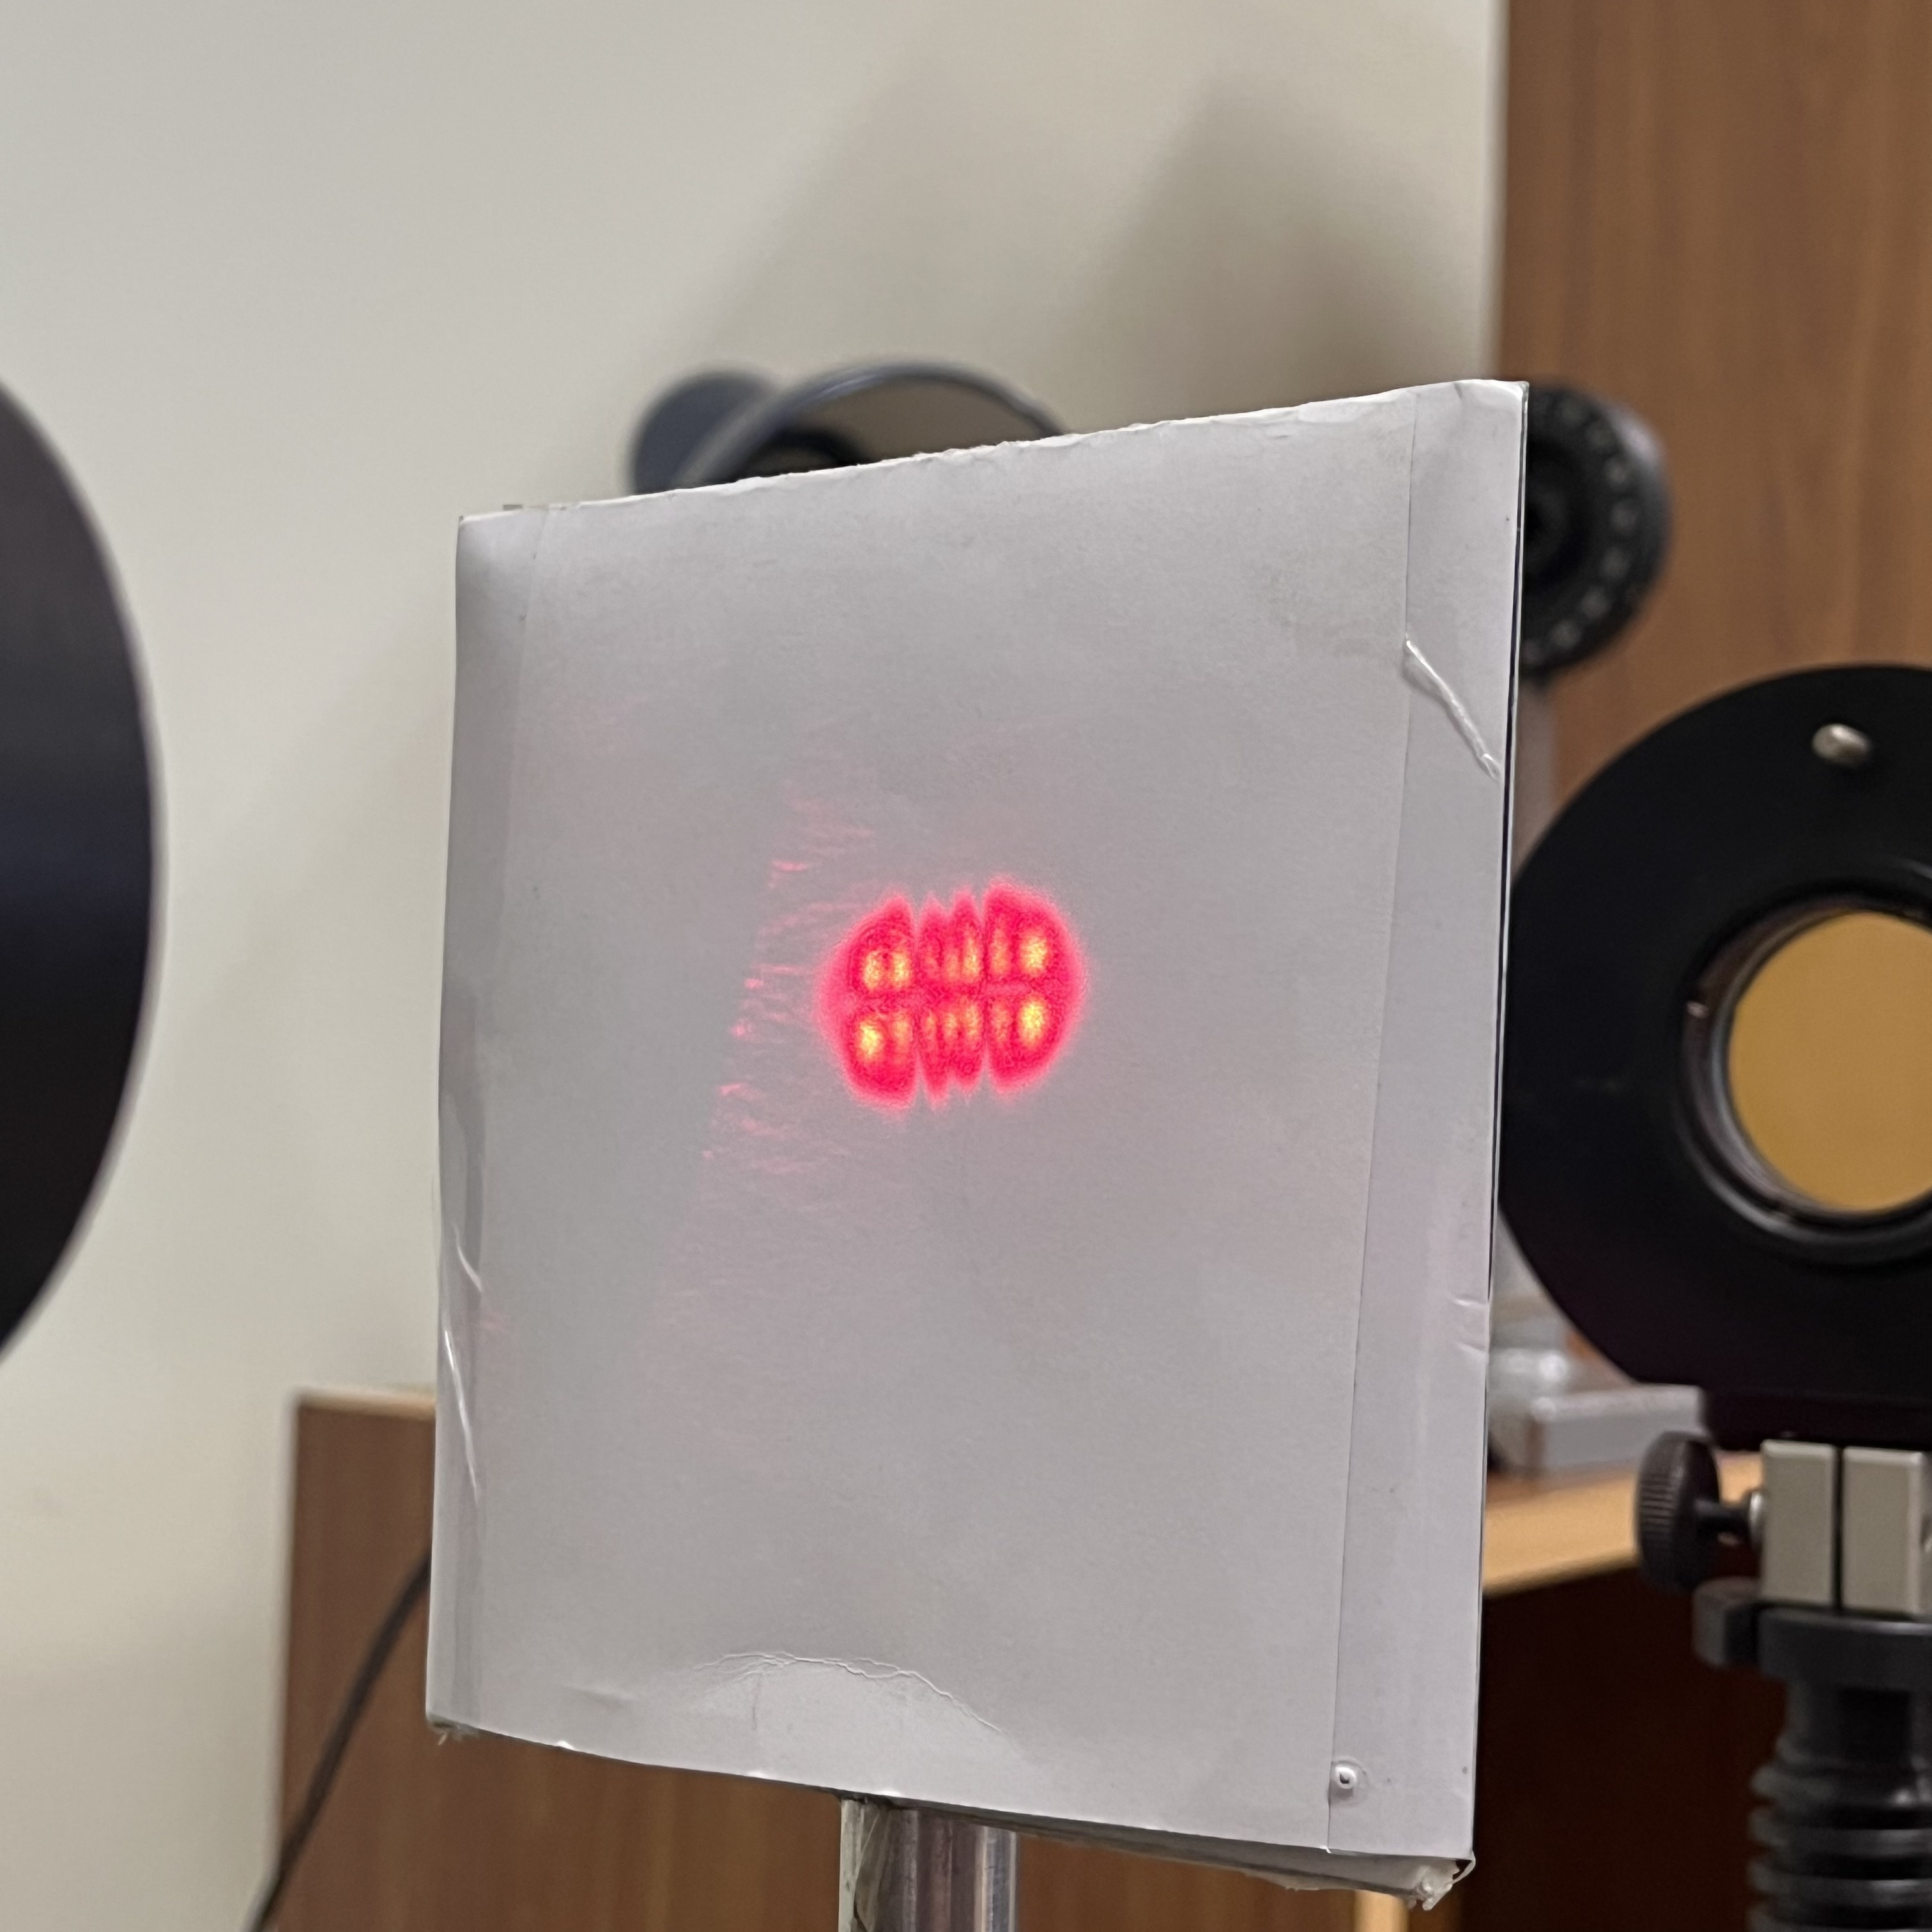
\includegraphics[width=1\linewidth]{5.JPG}}
		\caption{Многомодовый режим 3}
	\end{minipage}
	\begin{minipage}[h]{0.5\linewidth}
		\center{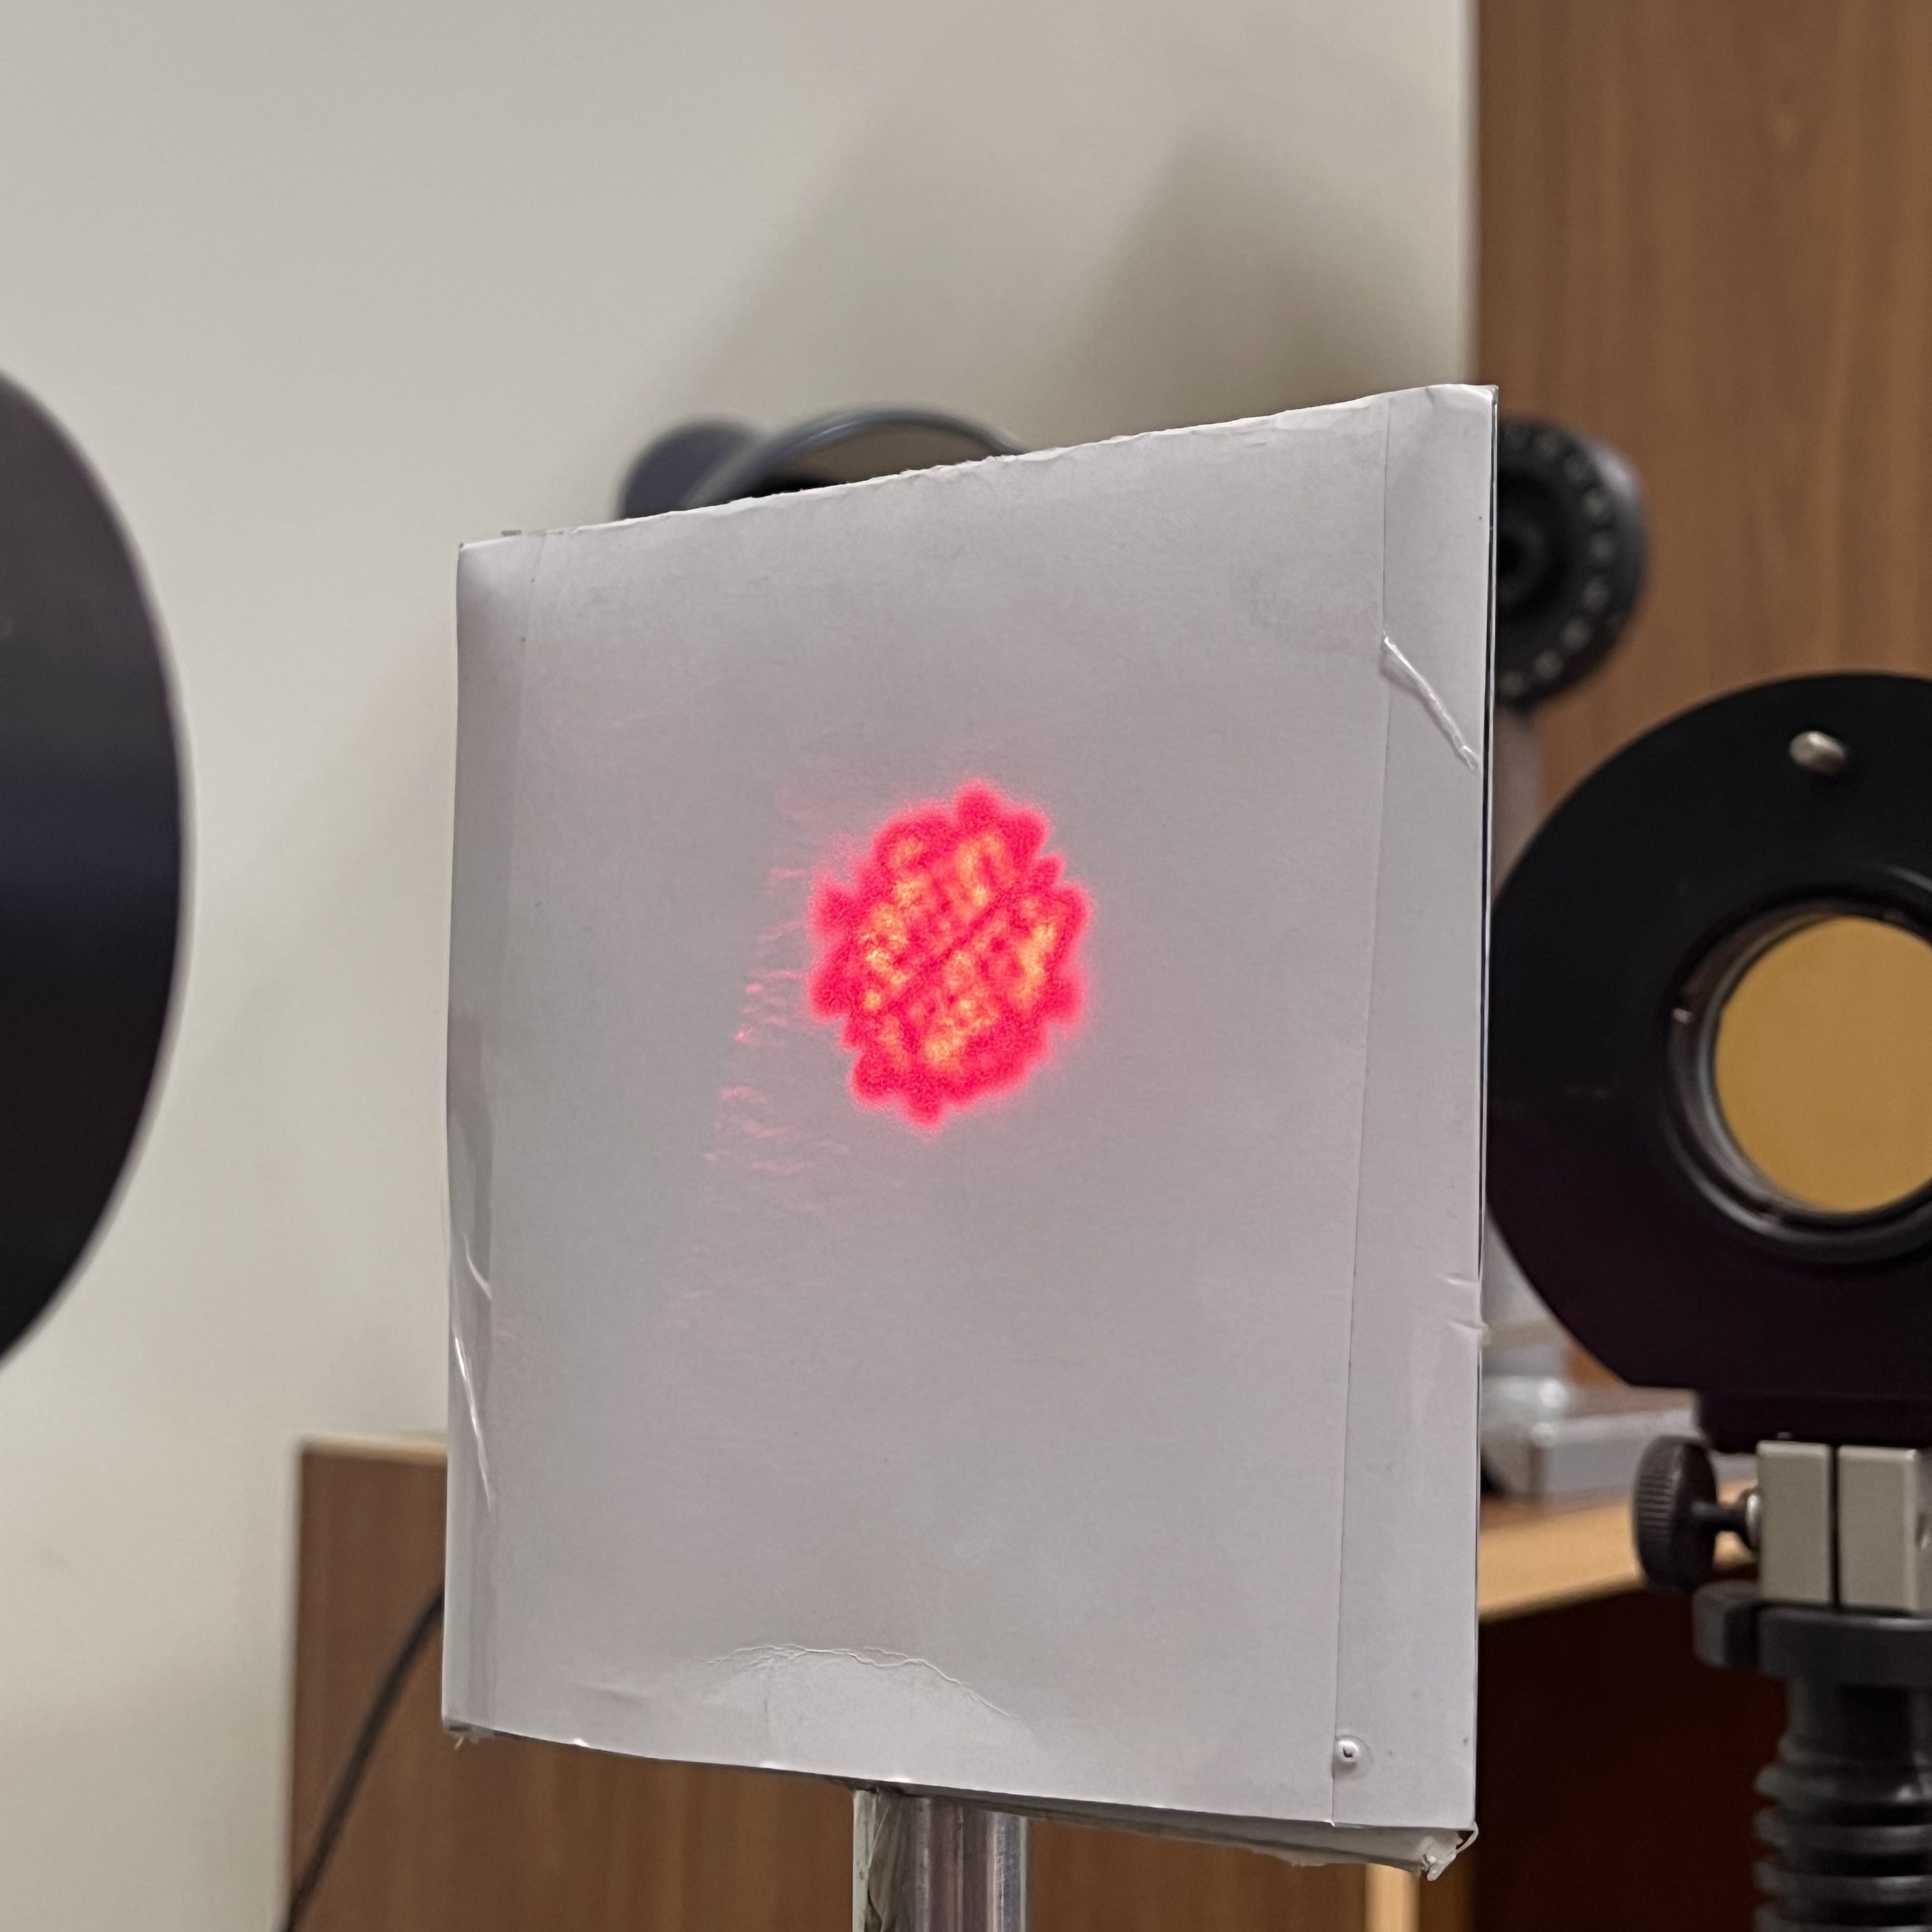
\includegraphics[width=1\linewidth]{6.JPG}}
		\caption{Многомодовый режим 4}
	\end{minipage}
\end{figure}

\subsection{Коэффициент усиления исследуемой трубки}
\par К сожалению, измерить коэффициент усиления не получилось ввиду неисправности установки. 
Согласно полученным на месте данным, усиление у трубки отсутствует, что очевидно противоречит
реальности.

\begin{figure}[H]
	\begin{minipage}[h]{0.49\linewidth}
		\center{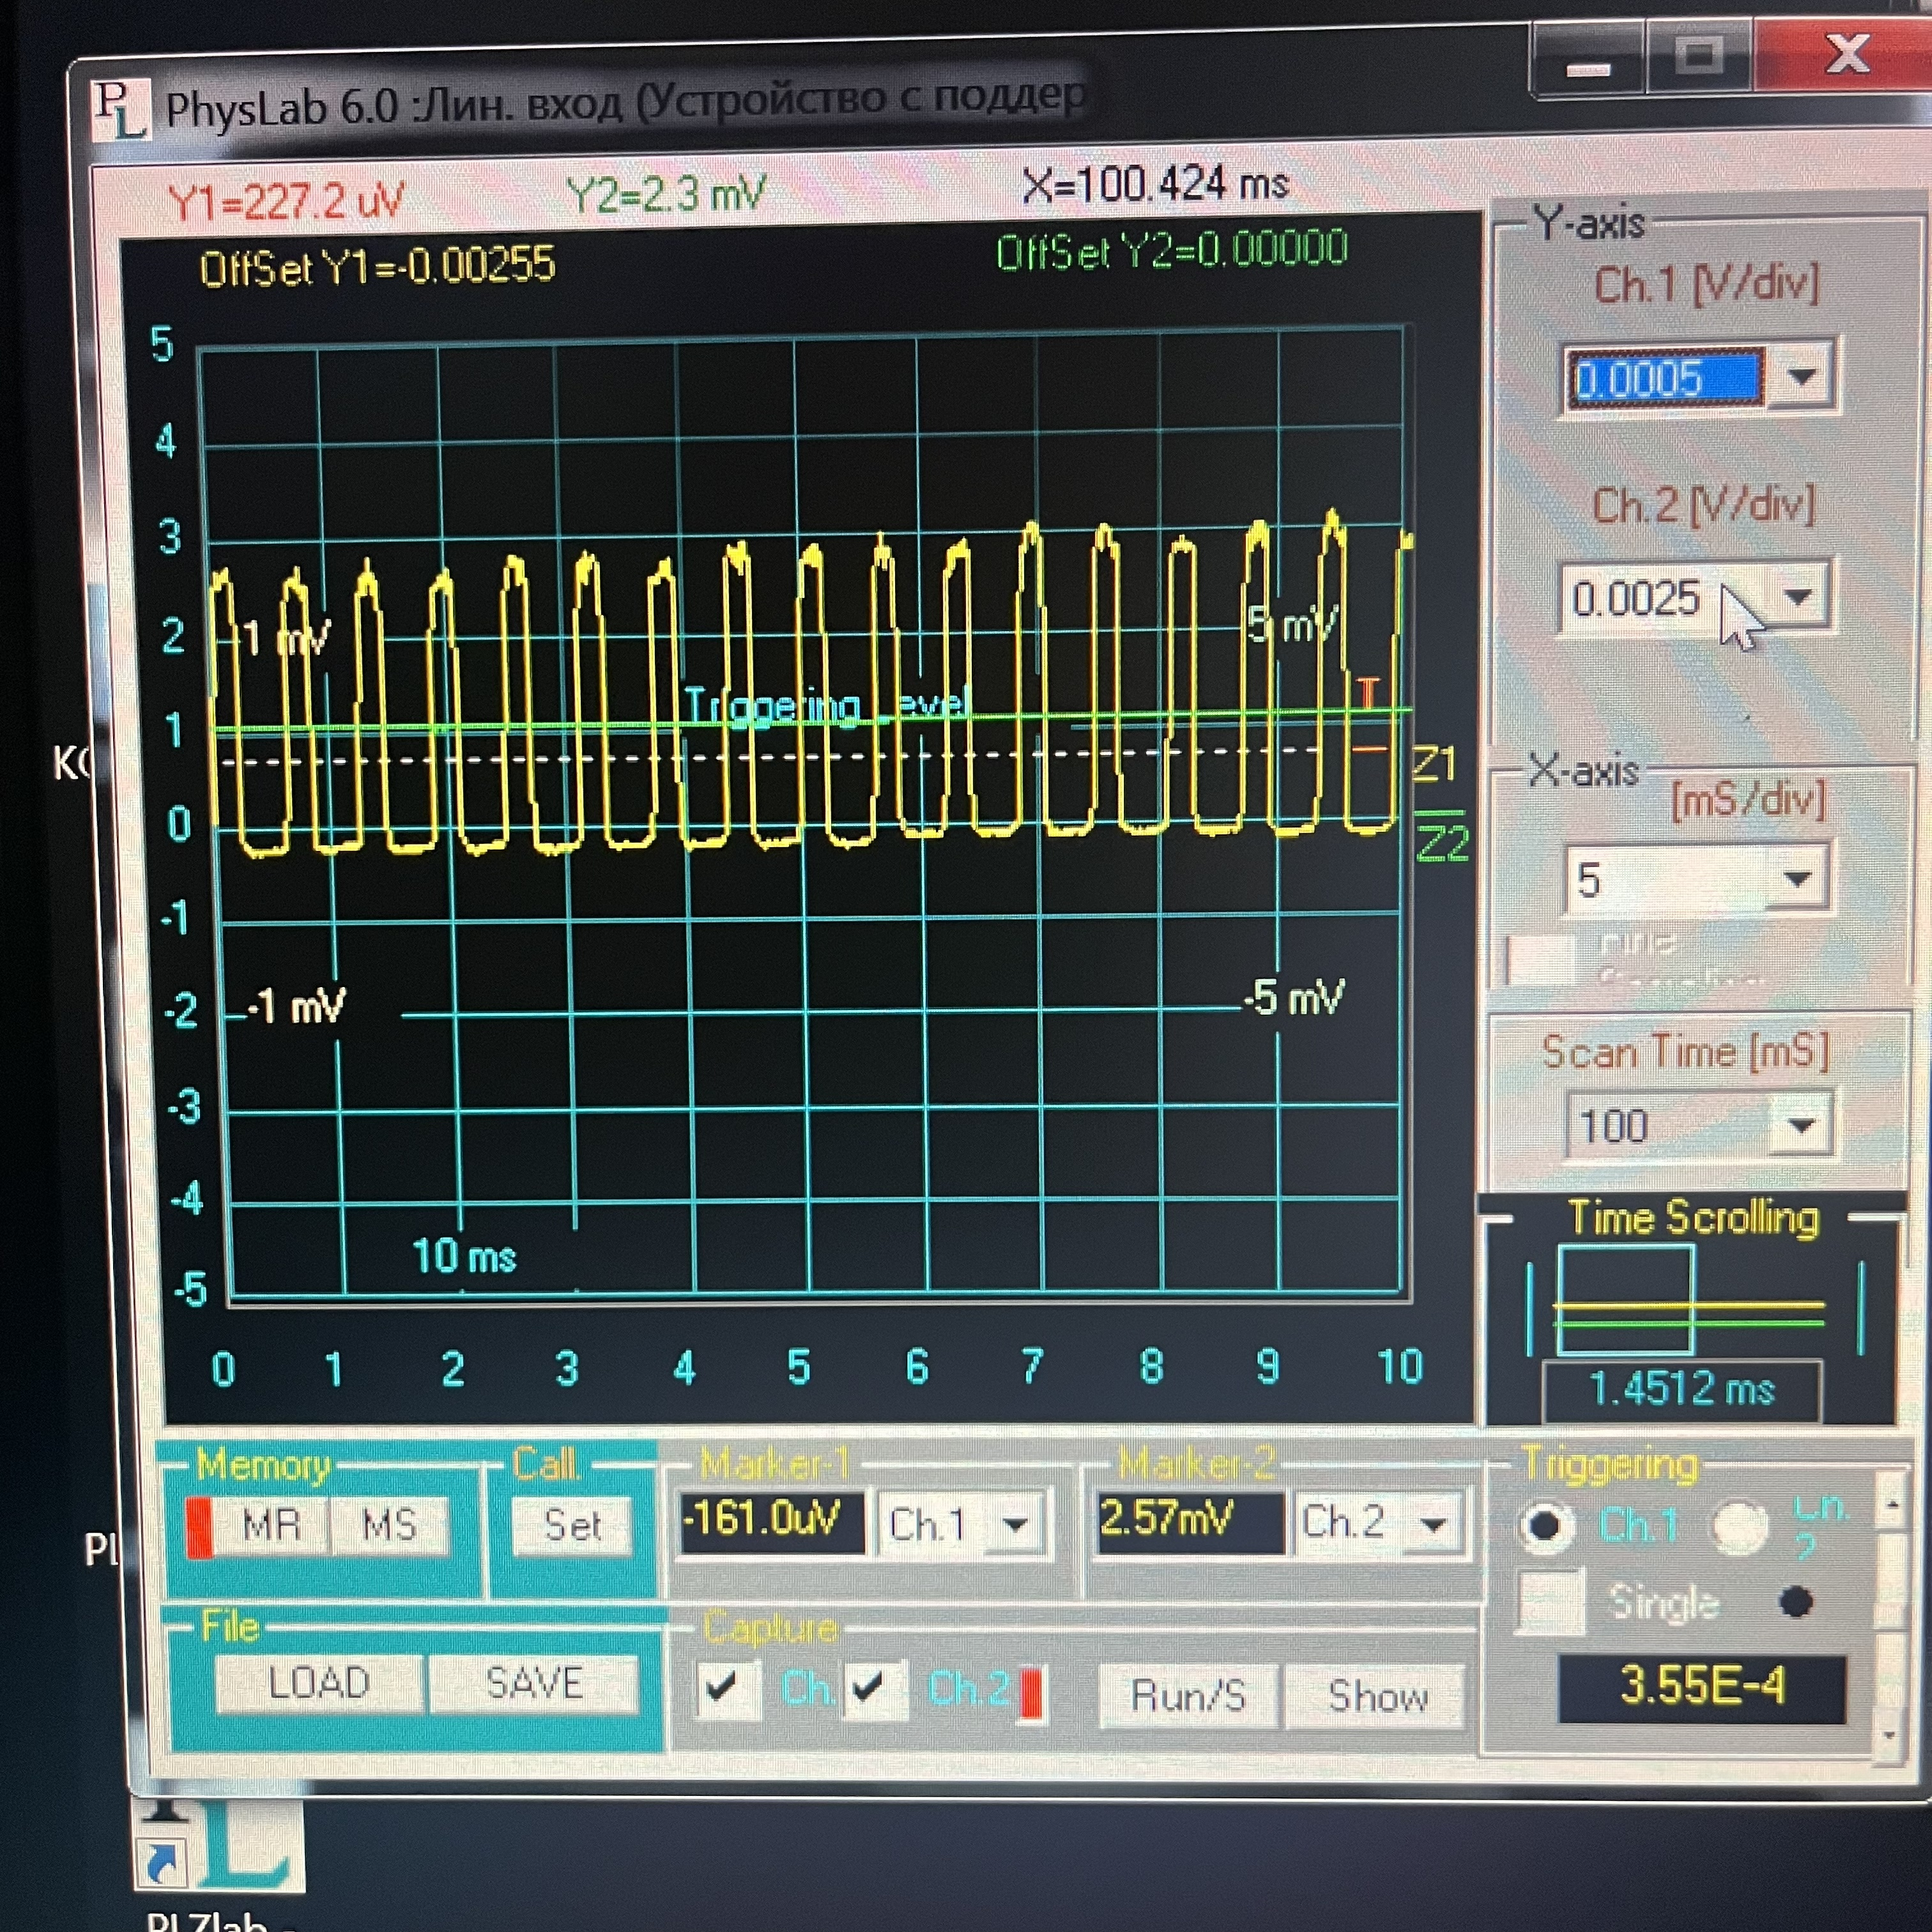
\includegraphics[width=0.95\linewidth]{physlab1.jpg}}
		\caption{Измерение интенсивности, программа PhysLab}
	\end{minipage}
	\begin{minipage}[h]{0.49\linewidth}
		\center{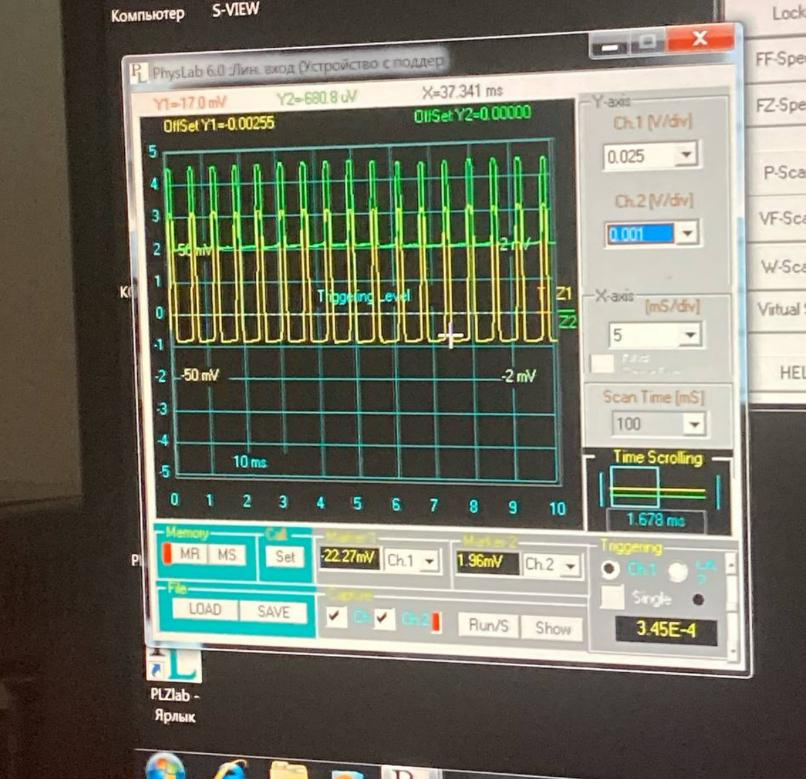
\includegraphics[width=0.95\linewidth]{physlab2.jpg}}
		\caption{Измерение коэффициента усиления, программа PhysLab}
	\end{minipage}
\end{figure}

\section{Вывод}

В данной работе были изучены основные принципы работы газового лазера и свойства лазерного излучения. Изучена поляризация лазерного излучения, была рассмотрена модовая структура лазерного излучения. Была совершена неудачная попытка получить коэффициент усиления исследуемой трубки.

\end{document}
